%%%%%%%%%%%%%%%%%%%%%%%%%%%%%%%%%%%%%%%%%%%%%%%%%%
% Basic setup. Most papers should leave these options alone.
\documentclass[a4paper,fleqn,usenatbib]{mnras}

% MNRAS is set in Times font. If you don't have this installed (most LaTeX
% installations will be fine) or prefer the old Computer Modern fonts, comment
% out the following line
\usepackage{newtxtext,newtxmath}
% Depending on your LaTeX fonts installation, you might get better results with one of these:
%\usepackage{mathptmx}
%\usepackage{txfonts}

% Use vector fonts, so it zooms properly in on-screen viewing software
% Don't change these lines unless you know what you are doing
\usepackage[T1]{fontenc}
\usepackage{ae,aecompl}


%%%%% AUTHORS - PLACE YOUR OWN PACKAGES HERE %%%%%

% Only include extra packages if you really need them. Common packages are:
\usepackage{graphicx}	% Including figure files
\usepackage{amsmath}	% Advanced maths commands
\usepackage{amssymb}	% Extra maths symbols
\usepackage{tikz}
\usepackage{enumerate}
\DeclareMathAlphabet{\mathcal}{OMS}{cmsy}{m}{n}
\usetikzlibrary{bayesnet}
%%%%%%%%%%%%%%%%%%%%%%%%%%%%%%%%%%%%%%%%%%%%%%%%%%

%%%%% AUTHORS - PLACE YOUR OWN COMMANDS HERE %%%%%

% Please keep new commands to a minimum, and use \newcommand not \def to avoid
% overwriting existing commands. Example:
%\newcommand{\pcm}{\,cm$^{-2}$}	% per cm-squared
\newcommand{\name}{Steve}
\newcommand{\myemail}{samuelreay@gmail.com}
\newcommand\abs[1]{\left|#1\right|}
\newcommand {\etal} {\emph{~et~al.} }
\newcommand{\green}{\color{green}}
\newcommand{\blue}{\color{blue}}
\newcommand{\red}{\color{red}}

\newcommand{\kmsmpc}{{\rm km}\,{\rm s}^{-1}\,{\rm Mpc}^{-1}}
\newcommand{\cov}{\mathcal{C}}
\newcommand{\Z}{\mathcal{Z}}

\defcitealias{Guy2010}{G10}
\defcitealias{Chotard2011}{C11}
\defcitealias{Rubin2015}{R15}	
\defcitealias{Scolnic2016}{SK16}	 
\newcommand{\gten}{\citetalias{Guy2010}}
\newcommand{\celeven}{\citetalias{Chotard2011}}
\newcommand{\rubin}{\citetalias{Rubin2015}}
\newcommand{\sk}{\citetalias{Scolnic2016}}
\newcommand{\angstrom}{\mbox{\normalfont\AA}}

\usepackage{lineno}
\linenumbers

\graphicspath{ {./figures/} }
%%%%%%%%%%%%%%%%%%%%%%%%%%%%%%%%%%%%%%%%%%%%%%%%%%

%%%%%%%%%%%%%%%%%%% TITLE PAGE %%%%%%%%%%%%%%%%%%%

% Title of the paper, and the short title which is used in the headers.
% Keep the title short and informative.
\title[\name]{\name: A hierarchical Bayesian model for Supernova Cosmology}

% The list of authors, and the short list which is used in the headers.
% If you need two or more lines of authors, add an extra line using \newauthor
\author[S. R. Hinton et al.]{
	Samuel R. Hinton,$^{1,2}$\thanks{E-mail: samuelreay@gmail.com}
	Alex G. Kim,$^{3}$
	Tamara M. Davis$^{1,2}$
	\\
	% List of institutions
	$^{1}$School of Mathematics and Physics, The University of Queensland, Brisbane, QLD 4072, Australia\\
	$^{2}$ARC Centre of Excellence for All-sky Astrophysics (CAASTRO)\\
	$^{3}$Physics Division, Lawrence Berkeley National Laboratory, 1 Cyclotron Road, Berkeley, CA 94720, USA
}

% These dates will be filled out by the publisher
\date{Accepted XXX. Received YYY; in original form ZZZ}

% Enter the current year, for the copyright statements etc.
\pubyear{2017}

% Don't change these lines
\begin{document}
\label{firstpage}
\pagerange{\pageref{firstpage}--\pageref{lastpage}}
\maketitle






% Abstract of the paper
\begin{abstract}
We present a hierarchical Bayesian model for use in supernova cosmology which takes into account a full range of analysis systematics and selection effects. This advances previous works with hierarchical Bayesian models by including additional sources of systematic uncertainty and improved treatment of Malmquist bias, whilst increasing numerical efficiency. Our model is optimised for efficient fitting and has been validated on a combined simulated dataset of more than $250\,000$ supernovae to rule out the presence of significant model biases in parameter recovery. Simplified statistical simulations for ideal supernovae cosmology show no bias, and sophisticated SNANA simulations of the combined low-redshift and DES 3-year spectroscopic survey sample quantify the bias for flat $w$CDM cosmology, with a matter prior $\Omega_m \sim \mathcal{N}(0.3, 0.01)$ included to allow rigorous determination of model bias in $w$. SNANA simulations can recover the input cosmology to within $0.27\sigma$, while taking into an increased number of systematics than prior analyses.
\end{abstract}
% Bias in SNANA tests across intrinsic dispersion models is found to range from $-0.15\sigma$ to $+0.27\sigma$ in $w$ for datasets of comparable strength to the Dark Energy Survey three-year analysis. 

% Select between one and six entries from the list of approved keywords.
% Don't make up new ones.
\begin{keywords}
keyword1 -- keyword2 -- keyword3\vspace{-5mm}
\end{keywords}









%%%%%%%%%%%%%%%%% BODY OF PAPER %%%%%%%%%%%%%%%%%%

\section{Introduction}




Almost two decades have passed since the discovery of the accelerating universe \citep{Riess1998, Perlmutter1999}. Since that time, the number of observed Type Ia supernovae (SNIa) have increased by more than an order of magnitude, with contributions from modern surveys at both low redshift \citep{Bailey2008, Freedman2009, Hicken2009,  Contreras2010, Conley2011}, and higher redshift \citep{Astier2006, Wood-Vasey2007, Frieman2008, Balland2009, Amanullah2010, Sako2014}. Cosmological analyses of these supernova samples \citep{Kowalski2008, Kessler2009, Conley2011, Suzuki2012, Betoule2014, Rest2014} have been combined with complimentary probes of large scale structureand the CMB. For a recent review, see \citet{Huterer2018}. Despite these prodigious efforts, the nature of dark energy remains an unsolved mystery.


In attempts to tease out the nature of dark energy, active and planned surveys are once again ramping up their statistical power. The Dark Energy Survey \citep[DES,][]{Bernstein2012, Abbott2016} has observed thousands of Type Ia supernova, attaining both spectroscopic and photometric selected samples. The Large Synoptic Survey Telescope \citep[LSST,][]{Ivezic2008, LSSTScienceCollaboration2009} will observe scores of thousands of photometrically classified supernovae. Such increased statistical power demands greater fidelity and flexibility in modelling the supernovae for cosmological purposes, as systematic uncertainties will prove to be the limiting factor in our analyses \citep{Betoule2014}.


As such, staggering effort is being put into developing more sophisticated supernova cosmology analyses. The role of simulations mimicking survey observations has become increasingly important in determining biases in cosmological constraints and validating specific cosmological models. First used in ESSENCE analyses \citep{Wood-Vasey2007}, and then refined and improved in \citet{Kessler2009}, simulations are now a fundamental component of modern supernovae cosmology.  \citet{Betoule2014} quantise and then correct observational bias using simulations, and more recently \citet{Scolnic2016} and \citet{Kessler2017} explore simulation to quantify observational bias in as a function of many factors to better remove fitting biases. Approximate Bayesian computation methods also make use of simulations, trading traditional likelihoods and analytic approximations for more robust models with the cost of increased computational time \citep{Weyant2013, Jennings2016}. Hierarchical Bayesian models abound \citep{Mandel2009, March2011, March2014, Rubin2015, Shariff2016, Roberts2017}, and either also use simulation corrections or attempt to find sufficient analytic approximations for complicated effects such as Malmquist bias.



In this paper, we lay out a new hierarchical model that builds off the past work of \citet{Rubin2015} to include more robust treatment of systematics and selection effects, whilst improving computational performance. Section \ref{sec:review} is dedicated to a quick review of the supernovae cosmology. In Section \ref{sec:method} we outline our methodology. Model verification on simulated datasets is given in Section \ref{sec:verification}, along with details on potential areas of improvement.



\section{Review}
\label{sec:review}

Whilst supernova observations take the form of time-series photometric measurements of brightness in many photometric bands, most analyses do not work from these measurements directly. Instead, most techniques fit and observed redshift and these photometric observations to a supernova model, with the most widely used being that of the empirical SALT2 model \citep{Guy2007, Guy2010}. This model is trained separately before fitting the supernovae light curves for cosmology \citep{Guy2010, Mosher2014}. The resulting output from the model is, for each supernova, a characterised amplitude $x_0$ (which can be converted into apparent magnitude $m_B = -2.5\log(x_0)$), a stretch term $x_1$ and colour term $c$, along with a covariance matrix describing the uncertainty on these summary statistics. As all supernova are not identical, an ensemble of supernova form a redshift-dependent, observed population of $m_B$, $x_1$ and $c$, where the width of this distribution is called the intrinsic dispersion of the supernova population.

The population previous discussed represents an observed population, which -- due to the presence of various selection effects -- may not represent the underlying supernova population. Accurately characterising this population, its evolution over redshift, and effects from environment, is one of the challenges of supernova cosmology. However, given some modelled underlying supernova population that lives in the redshift-dependent space $M_B$ (absolute magnitude), $x_1$ and $c$, the introduction of cosmology into the model is simple -- it is encoded in the functional map between those two populations, from apparent magnitude space to absolute magnitude. Specifically, for any given supernova our functional map may take the traditional form:

\begin{align}
M_B = m_B + \alpha x_1 - \beta c - \mu(z) + \text{other corrections}, \label{eq:standard}
\end{align}

where $M_B$ is the mean absolute magnitude for all SN Ia  $\alpha$ is the stretch correction \citep{Phillips1993, Phillips1999}, and $\beta$ is the colour correction \citep{Tripp1998} that respectively encapsulate the empirical relation that broader (longer-lasting) and bluer supernovae are brighter. The cosmological term, $\mu(z)$ represents the distance modulus, and is precisely known given cosmological parameters and a redshift. The $\text{other corrections}$ term often includes corrections for host galaxy environment, as this has statistically significant effects on supernova properties \citep{Kelly2010, Lampeitl2010, Sullivan2010, DAndrea2011, Gupta2011, Johansson2013, Rigault2013, Uddin2017} In traditional analyses, the other corections term often includes bias corrections, which can take the form of a redshift-dependent function \citep{Betoule2014}.

\subsection{Traditional Cosmology Analyses}

Traditional $\chi^2$ analyses such as that found in \citet{Riess1998, Perlmutter1999, Wood-Vasey2007, Kowalski2008, Kessler2009, Conley2011, Betoule2014}, minimise the difference in distance modulus between the observed distance modulus $\mu_{\rm obs}$ (attained from rearranging equation \eqref{eq:standard}), and the cosmologically predicted values $\mu_C$. This function is given by

\begin{align}
\chi^2 = (\mu_{\rm obs} - \mu_C)^\dagger C^{-1} (\mu_{\rm obs} - \mu_C),
\end{align}

where $C^{-1}$ is an uncertainty matrix that combines the uncertainty from the SALT2 fits, intrinsic dispersion, calibration, dust, peculiar velocity and many other factors (see \citet{Betoule2014} for a review). The cosmological $\mu_C$ is defined as

\begin{align}
\mu_C &= 5 \log\left[ \frac{(1+z)r}{10} \right],\\
r& =\frac{c}{H_0} \int_0^z \frac{dz'}{\sqrt{ \Omega_m (1+z')^3 + \Omega_k (1 + z')^2 + \Omega_\Lambda (1+z')^{3(1+w)}}}, \label{eq:mu0}
\end{align}
where $r$ is the comoving distance for redshift $z$ given a specific cosmology and $H_0$ is the current value of Hubble's constant in $\kmsmpc$.

The benefit this analysis methodology provides is speed -- for samples of hundreds of supernovae or less, efficient matrix inversion algorithms allow the likelihood to be evaluated quickly. The speed comes with several limitations. Firstly, formulating a $\chi^2$ likelihood requires a loss of model flexibility by building into the model assumptions of Gaussian uncertainty. Secondly, the method of creating a global covariance matrix relies on computing partial derivatives and thus any uncertainty estimated from this method loses all information about correlation between sources of uncertainty. For example, the underlying supernova colour population's mean and skewness is highly correlated, however this correlation is lost when determining population uncertainty using numerical derivatives of population permutations. Thirdly, the computational efficiency is dependent on inverting a covariance matrix with dimensionality linearly proportional to the number of supernovae. As this number increases, the cost of inversion rises quickly, and is not viable for samples with thousands of supernovae. A common solution to this computational cost problem is to bin the supernova.

Selection efficiency, such as the well known Malmquist bias \citep{MalmquistK.G.1922} is accounted for by correcting data. Specifically, Malmquist bias is the result of losing the fainter tail of the supernova population at high redshift when supernovae increasingly fall below the detection threshold. An example of Malmquist bias is illustrated in Figure \ref{fig:malmquist}. Simulations following survey observational strategies and geometry are used to calculate the expected bias in distance modulus, which is then added onto the observational data. As these effects are not built into the likelihood and instead are formed by correcting data, their uncertainty is not captured fully in the $\chi^2$ distribution, and any subtle correlations between cosmological or population parameters and the bias is lost.

\begin{figure}
	\begin{center}
		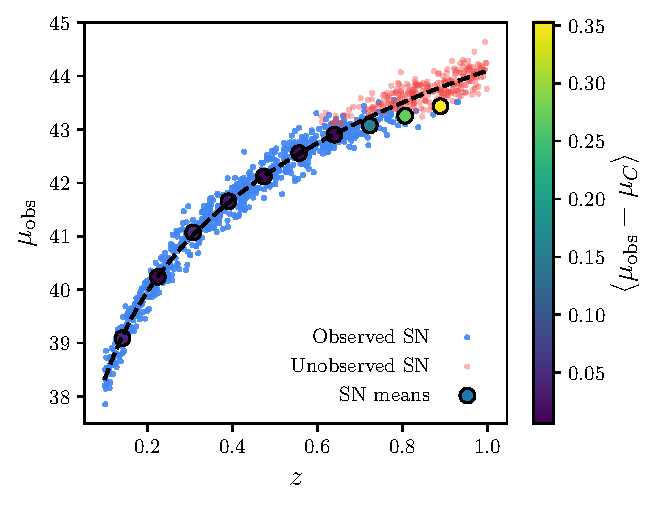
\includegraphics[width=\columnwidth]{malmquist.pdf}
	\end{center}
	\caption{An example of the effects of Malmquist bias. Here are shown 1000 simulated supernovae redshifts and distance modulus given fiducial cosmology. The simulated survey is magnitude limited, and all supernovae brighter than magnitude 24 are successfully observed (shown as blue dots), and all dimmer than 24th magnitude are not successfully observed (shown as red dots). By binning the supernovae along redshift, and taking the mean distance modulus of the supernovae in each bin, we can see that at higher redshift where Malmquist bias kicks in, the population mean drops and becomes bias. This source of bias must either be corrected by adjusting the data (such as subtracting the found bias) for by incorporating Malmquist bias explicitly in the cosmological model.}
	\label{fig:malmquist}
\end{figure}


\subsection{Approximate Bayesian Computation}

To try and escape the limitations of the traditional approaches, several recent methods have adopted Approximate Bayesian Computation, where supernova samples are forward modelled in parameter space and compared to observed distributions. \citet{Weyant2013} provides an introduction into ABC methods for supernova cosmology in the context of the SDSS-II results \citep{Sako2014} and flat $\Lambda$CDM cosmology, whilst \citet{Jennings2016} demonstrates their \textit{superABC} method on simulated first season Dark Energy Survey samples, described in \citet{Kessler2015}. In both examples, the supernova simulation package SNANA \citep{Kessler2009a} is used to forward model the data at each point in parameter space.

Simulations provide great flexibility and freedom in how to treat the systematic uncertainties and selection effects that plague supernovae surveys. By using forward modelling directly from these simulations, data does not need to be corrected, analytic approximations do not need to be applied; we are free to incorporate algorithms that simply cannot be expressed in a tractable likelihood. This freedom comes with a cost -- computation. The classical $\chi^2$ method's most computationally expensive step in a fit is matrix inversion. For ABC methods, we must instead simulate an entire supernova population -- drawing from underlying supernova populations, modelling light curves, applying selection effects, fitting light curves and applying data cuts. This is an intensive process.

One final benefit of ABC methods is that they can move past the traditional treatment of supernovae with summary statistics ($m_B$, $x_1$ and $c$). \citet{Jennings2016} presents both two metrics (which are used to measure the distance between the forward modelled population and observed population, which is minimised in fitting). The first metric compares forward modelled summary statistic populations (denoted the `Tripp' metric) and the second utilises the observed supernova light curves themselves, moving past summary statistics. However, we note that evaluation of systematic uncertainty was only performed using the Tripp metric.

\subsection{Hierarchical Bayesian Models}

Sitting between the traditional models simplicity and the complexity of forward modelling lies Bayesian hierarchical models (BHM). Hierarchical models utilise multiple layers of connected parameters in their models, with the layers linked via well defined and physical motivated conditional probabilities. For example, an observation of a parameter from a population will be conditioned on the true value of the parameter, which itself will be conditioned on the population distribution of that parameter. We can thus easily incorporate different distributions, populations, and parameter inter-dependence which cannot be found in traditional analyses where uncertainty must be encapsulated in a covariance matrix.

With the introduction of multiple layers in our model, we can add far more flexibility than a traditional analysis whilst still maintaining most of the computational benefits that come from having a tractable likelihood. \citet{Mandel2009, Mandel2011a, Mandel2017} construct a hierarchical model that they apply to supernova light curve fitting. \citet{March2011} derive a hierarchical model and simplify it by analytically marginalising over nuisance parameters to provide increased flexibility with reduced uncertainty over the traditional method, but does not incorporate bias correction. \citet{March2014, Karpenka2015} improve upon this by incorporating redshift-dependent magnitude corrections from \citet{Perrett2010} to remove bias, and validate on 100 realisations of SNLS like simulations. The recent BAHAMAS model \citep{Shariff2016} builds on this and reanalyses the JLA dataset (using their redshift dependent bias corrections), whilst including extra freedom in the correction factors $\alpha$ and $\beta$, finding evidence for redshift dependence on $\beta$. \citet{Ma2016} performed a reanalysis of the JLA dataset within a Bayesian formulation, finding significant differences in $\alpha$ and $\beta$ values from the original analysis from \citet{Betoule2014}. Notably, these methods rely on data that is bias corrected or ignore biases, however the UNITY framework given by \citet{Rubin2015} incorporates selection efficiency analytically in the model, and is applied to the Union 2.1 dataset \citep{Suzuki2012}. The simplification made by the UNITY analysis is that the bias is well described by an analytic function, and this function is fixed such that selection effects are assumed to be determined with perfect precision. Their model was validated to be free of significant biases using fits to thirty realisations of statistics. 

Whilst there are a large amount of hierarchical models available, all so far mentioned, in the case where any validation has been done, have been done on either $\Lambda$CDM cosmology or Flat $\Lambda$CDM cosmology. None of them have undergone high-statistics simulation verification for $w$CDM cosmology to quantify each models' respective bias, which is becoming critically important as precision supernovae cosmology comes into its own and focus shifts from determination of $\Omega_m$ to $w$.

The well known BEAMS (Bayesian estimation applied to multiple species) methodology from \citet{Kunz2007} has been extended and applied in several works \citep{Hlozek2012}, mostly lately to include redshift uncertainty for photometric redshift application as zBEAMS \citep{Roberts2017} and to include simulated bias corrections in \citet{Kessler2017}. For the latter case, by inferring biases using Bayesian models, sophisticated corrections can be calculated and then applied to more traditional $\chi^2$ models.

The flexibility afforded by a hierarchical model allows for investigations into different treatments of underlying supernova magnitude, colour and stretch populations, supernovae rates and redshift distributions, and host-galaxy corrections and redshift evolution, each of which will be discussed further in the outline of our model below. 









\section{Our Method}
\label{sec:method}

We construct our hierarchical Bayesian model with several goals in mind: creation of a redshift-dependent underlying supernova population, increased treatment of systematics, and analytic correction of selection effects, including systematic uncertainty on those corrections. We also desire this to be more computationally efficient than prior works, such that cosmological results from thousands of supernovae are obtainable in the order of hours, rather than days. As this is closest to the UNITY method from \citet[][hereafter denoted \rubin]{Rubin2015}, we follow a similar model scaffold, and construct the model in Stan \citep{Carpenter2017, StanDevelopmentTeam2017}. The primary challenge of fitting hierarchical models is their large number of fit parameters, and Stan, which uses automatic differentiation and the no-U-turn Sampler (NUTS) (a variant of Hamiltonian Monte Carlo), allows us to efficiently sample high dimensional parameter space.

At the most fundamental level, a supernova analysis is simply a mapping from an underlying population onto an observed population, where cosmology is encoded directly in the mapping function. The difficulty arises both in adequately describing the biases in the mapping function, and in adding sufficient, physically motivated flexibility in both of these populations whilst not adding \textit{too} much flexibility, such that model fitting becomes pathological due to increasing parameter degeneracies within the model. In the following sections, we will describe these layers, mapping functions, and occurrences of these fatal pathologies.


\subsection{Observed Populations}

Like most of the BHM methods introduced previously, we work from the summary statistics, where each observed supernova has an apparent magnitude $\hat{m}_B$, stretch $\hat{x}_1$ and colour $\hat{c}$, with uncertainty $\cov$ on those values. Additionally, each supernova has an observed redshift $\hat{z}$ and a host galaxy mass associated with it, $\hat{m}$, where the mass measurement takes the form of a probability of being above $10^{10}$ solar masses. We will also have a probability of being a Type Ia, $\hat{p}$. Our set of observables is therefore given as $\lbrace \hat{m}_B, \hat{x}_1, \hat{c}, \hat{z}, \hat{p}, \hat{m}, \cov \rbrace$, as shown in the probabilistic graphical model (PGM) in Figure \ref{fig:pgm}.


As we are focused on the spectroscopically confirmed supernovae for this iteration of the method, we assume the observed redshift $\hat{z}$ is the true redshift $z$ such that $P(\hat{z}|z) = \delta(\hat{z} - z)$. Potential sources of redshift error (such as peculiar velocities) is taken into account not via uncertainty on redshift (which is technically challenging to implement) but instead uncertainty on distance modulus. This is discussed further in Section \ref{sec:systreat}. Similarly, we take the mass probability estimate $\hat{m}$ as correct, and do not model a latent variable. One of the strengths of this model (and the {\rubin} analysis) is that for future data sets where supernovae have been classified photometrically, and we expect some misclassification and misidentification of the host galaxies, those can naturally be modelled and taken into account.

The first layer of the hierarchy represents the parameters that describe each supernova. That is, observed parameters are denoted with a hat, whilst the true value is denoted without a hat. For example, $c$ is the true colour of the supernova, whilst $\hat{c}$ is the colour we observe, which, as it has uncertainty, is different from $c$.

For the moment, let us consider a single supernova, and represent its true parameters as $\theta$. The underlying supernova model and intrinsic dispersion model gives the probability of $p(y|\theta)$ for obtaining light curve data $y$. As mentioned earlier, we work with summary statistics -- numbers output from a light curve fitter given the input $y$. The function $f$ describes the action of the fitter $\lbrace \hat{m}_B, \hat{x}_1., \hat{c} \rbrace = f(y)$. For notational simplicity, let us denote $\eta \equiv \lbrace m_B, x_1, c \rbrace$. The model prediction for our derived data is

\begin{align}
p(\hat{\eta} | \theta) = \int \delta(\hat{\eta} - f(y)) p(y | \theta) \, dy.
\end{align}

To help confuse things, we often consider models that are parametrised as $\theta = \lbrace m_B, x_1, c \rbrace = \eta$, so that the probability of derived data is expressed as

\begin{align}
p(\hat{\eta}|\eta) = \int \delta(\hat{\eta} - f(y)) p(y|\eta) dy. \label{eq:intsmear}
\end{align}

It is common in analytic supernova cosmology models to take that

\begin{align}
p(\hat{\eta}|\eta) \sim \mathcal{N}(\hat{\eta} | \eta, \mathcal{C}), \label{eq:pop}
\end{align}

where $\mathcal{C}$ is a covariance matrix reported from light curve fitting. Unfortunately, this assumption of Gaussianity is incorrect. The intrinsic supernovae population is commonly described in terms of coherent magnitude dispersion, wherein some supernovae are uniformly brighter or dimmer than the population mean, and in chromatic dispersion, whereby the spectral energy density of the supernovae varies non-uniformly as a function of wavelength. The presence of chromatic smearing in the intrinsic supernova population \citep{Guy2010, Chotard2011} means the summary statistics reported from light curve fitting are under-reported, not Gaussian and equation \eqref{eq:pop} is violated. We address this problem with a similar method to previous analytic likelihoods: including extra dispersion in the reported covariance matrix $\mathcal{C}$. Whilst this doesn't solve the issue of non-Gaussianity, it does address the under-reporting of uncertainty, which is the primary source of bias.

We model the extra dispersion only in colour, and do so by adding extra independent uncertainty on the colour observation. Fully covariant extra dispersion on $\lbrace m_B, x_1, c \rbrace$ was also tested, but it showed negligible improvement over just colour dispersion and was far more computationally inefficient. As shown in \citep{Kessler2013}, the extra colour dispersion shows heavy redshift dependence. As the extra dispersion may arise from underlying supernova physics, rather than Malmquist bias, we decide to incorporate redshift dependence in our extra uncertainty. We thus add $\kappa_0 + \kappa_1 z$ to our observed colour uncertainty (in quadrature), where $\kappa_0$ and $\kappa_1$ are subject to strong Cauchy priors centered on zero and with width $0.002$, to enforce minimum possible extra uncertainty in our model. The $\kappa$ parameters are tightly constrained as they are highly degenerate with the width of the intrinsic colour population $\sigma_c$, and the specific value of this prior was determined from running many iterations of simulation fitting with differing prior strengths on our simple data set with simulated extra dispersion according to the results of \citet{Kessler2013}. The value $0.002$ can be varied by a factor of approximately three in either direction whilst giving stable results, with larger values (more than a factor of three) for the prior resulted in incorrect determination of $\sigma_c$, whilst smaller values resulted in being unable to capture the extra dispersion  Each survey has its own set of $\kappa$ parameters. As such, our combined covariance on the observation $\hat{\eta}$ is given by $\mathcal{C}_{\rm tot} = \mathcal{C} + {\rm DiagMatrix}\left[0, 0, (\kappa_0 + \kappa_1 z)^2\right]$.


Furthermore, we use fiducial simulations (discussed further in Section \ref{sec:selection}) to characterise the shift in the mean colour measured as a function of redshift, and subtract this shift from our observed data. With the extra dispersion introduced from the $\kappa$ parameters addressing the under-reporting of error, shifting the mean colour address the non-Gaussianity introduced by chromatic smearing. We allow the amount of shift to be parametrised to account for different intrinsic scatter models where parameter $s_c$ controls the fraction of bias subtraction -- 0 for no shift, up to 1 for the maximum shift found in simulations. The scatter models, sourced from \citet{Guy2010} and \citet{Chotard2011} are discussed in detail in Section \ref{sec:simdes}. The maximum shift was found to using the intrinsic scatter model from \citet{Chotard2011}. Unlike $\kappa_0$ and $\kappa_1$, which are redefined for each survey, $s_c$ represents a global shift in supernovae colour across all surveys. We place a uniform prior on $s_c$. It is important to note that the effects being modelled and characterised by simulations here are features of the supernova population, not cosmological features, and so the choice of fiducial cosmology has negligible impact.

 \begin{figure}
	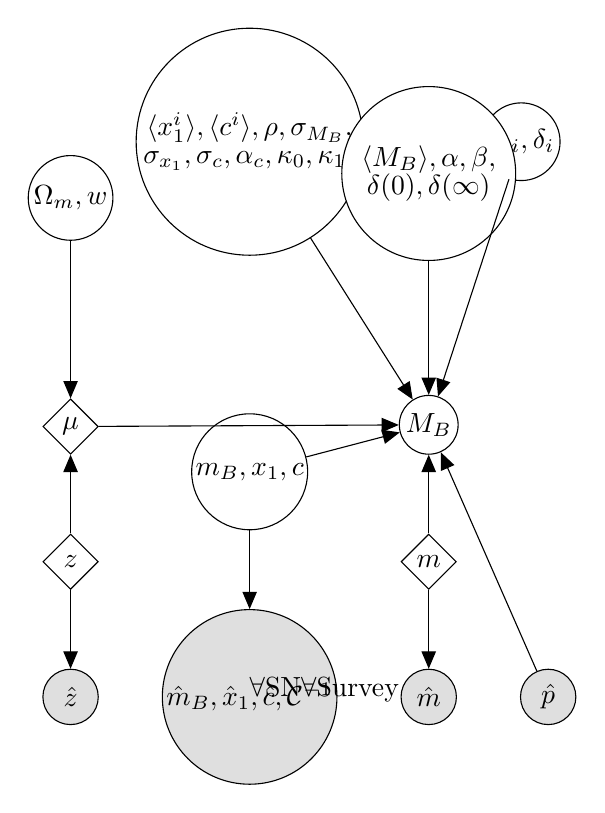
\begin{tikzpicture}
	% Obs nodes
	\node[obs]  (obssum) {$\hat{m}_B, \hat{x}_1, \hat{c}, \mathcal{C}^{-1}$};
	\node[obs, left=0.8cm of obssum]  (zobs) {$\hat{z}$};
	\node[obs, right=0.8cm of obssum]  (mobs) {$\hat{m}$};
	\node[obs, right=0.8cm of mobs]  (pobs) {$\hat{p}$};
	
	% Latent nodes
	\node[latent, above=of obssum] (sum) {$m_B, x_1, c$};
	\node[det, above=of zobs] (z) {$z$};
	\node[det, above=of mobs] (m) {$m$};
	\node[det, above=of z] (mu) {$\mu$};
	\node[latent, above=of m] (MBobs) {$M_B$};
	% Survey nodes
	\node[latent, above=of sum, yshift=1cm,text width=2.7cm, align=center] (pop1) {$\langle x_1^i \rangle, \langle c^i \rangle,\rho,\sigma_{M_B}, $\\$ \sigma_{x_1}, \sigma_c, \alpha_c, \kappa_0, \kappa_1, s_c$ };
	\node[latent, right=1.5cm of pop1, align=center] (sf) {$\Delta_i, \delta_i$};
	% Global nodes
	\node[latent, above=2cm of mu]  (cosmo) {$\Omega_m, w$};
	\node[latent, above=1.7cm of MBobs, text width=2cm, align=center]  (ab) {$\langle M_B \rangle, \alpha, \beta,$\\$\delta(0), \delta(\infty)$};
	
	% Connect the nodes
	\edge {sum} {obssum};
	\edge {z} {zobs};
	\edge {m} {mobs};
	\edge {z,cosmo} {mu};
	\edge {mu, sum, m, pop1, ab, pobs, sf} {MBobs};
	
	% Plates
	\plated[thick] {sn} {(obssum)(zobs)(mobs)(pobs)(sum)(z)(m)(mu)} {$\forall\ \rm{SN}$} ;
	\plated[thick] {survey} {(sn)(pop1)} {\\$\forall\ \rm{Survey}$} ;
	\end{tikzpicture}
	\caption{Probabilistic graphical model for our likelihood. Double-lined nodes represent observed variables, diamond nodes represent deterministic variables, and standard nodes represent fit variables. The SN box represents observed variables and latent variables for each individual supernova, whilst the survey box represents survey-specific variables, which in general describe the supernova population for the survey and the systematics associated with it.}
	\label{fig:pgm}
 \end{figure}


\subsection{Underlying Population}

The underlying supernova population is characterised by underlying distributions in colour, stretch and absolute magnitude. Analytic models often treat the colour and stretch populations independently with a skew normal and normal, respectively. Intrinsic dispersion is treated in a variety of manners in other models, from representing it simply as (Gaussian) scatter on the absolute magnitude of the supernova population, to correlated multivariate normal scatter on the combined magnitude, stretch and colour distribution. Additionally, redshift drift of populations' mean colour and stretch will introduce a cosmological bias in our fits unless the model population possesses similar ability to change as a function of redshift. 

We follow prior work and model the colour population as an independent redshift-dependent skew normal for each survey. For the stretch population, we adopt a redshift-dependent normal, and magnitude dispersion is modelled as a normal. Following {\rubin} we allow the mean colour and stretch to vary over redshift, anchoring four equally spaced redshift nodes spanning the redshift range of each survey, linearly interpolating between the nodes. Each set of nodes are anchored to equally spaced to span the minimum to maximum redshift of each survey. These nodes are represented as $\langle x_1^i \rangle$ and $\langle c^i \rangle$. Both the colour and stretch means are modelled with normal priors. Initial versions of our model adopted a fully covariant multivariate skew normal (with skewness set to zero only for the magnitude component), however pathological fitting complications required us to simplify our treatment. We parameterise the skewness $\alpha_c$ by sampling $\delta_c = \alpha_c / \sqrt{1 + \alpha_c^2}$ which itself is given a uniform prior $\mathcal{U}(0,0.98)$, which allows $\alpha_c$ to span positive values in the realm of physical plausibility as determined from constraints in \citet{Scolnic2016}. The width of the population, represented by the vector $\lbrace \sigma_{M_B}, \sigma_{x_1}, \sigma_c \rbrace$ is subject to Cauchy priors, however are sampled in log space for efficiency in sampling close to zero. 

As such, the only constant between survey populations is the mean absolute magnitude $\langle M_B \rangle$, with the skewness, redshift-dependent means and width fit individually for each survey. The probability for a supernova to have true values $M_B$, $x_1$, $c$ given the underlying population is thus given as

\begin{align}
P(M_B, x_1, c, z | \langle M_B \rangle, \langle x_1(z) \rangle, \langle c(z) \rangle, \sigma_{m_B}, \sigma_{x_1}, \sigma_c, \alpha_c) = \notag \\
\mathcal{N}(M_B|\langle M_B \rangle, \sigma_{M_B}) \mathcal{N}(x_1 | \langle x_1(z) \rangle, \sigma_{x_1}) \mathcal{N}^{\rm{skew}}(c| \langle c(z) \rangle, \sigma_c, \alpha_c) \label{eq:l1}.
\end{align}


On top of the SNIa populations, as described above, we also include a simplistic outlier population that also follows {\rubin} \citep[and therefore ][]{Kunz2007} as a Gaussian mixture; where the mean of the population is fixed to the SNIa population, but the population width is set to a width of $\sigma^{\rm outl} = 1$ in $M_B$, $x_1$ and $c$. With the spectroscopic DES sample, the contamination rate is expected to be far too low to actually fit contamination population, however in future works with photometric samples that will suffer from significantly more contamination, it will be required that extra degrees of freedom are afforded the outlier population. This contamination is not just a result of non-SNIa being observed, but can also arise from host galaxy misidentification and incorrect redshifts - depending on the cuts on the optimised ratio between purity and efficiency, this can result in between 3\% to 9\% misidentification  \citep{Gupta2016}. Proof of concept analysis on simple simulation data show that an acceptable parametrisation to deal with contamination, both from non type Ia supernovae and from catastrophic failure, is to represent the typically dimmer contaminant population as $\langle M_B^{\rm outl} \rangle = \langle M_B \rangle + \delta_{M_B}^{\rm outl}$, where $\delta_{M_B}^{\rm outl}$ is constrained to be positive, or even to be greater than a small positive number to reduce degeneracy between the two populations. For the purposes of the DES spectroscopic sample, which will be confirmed SNIa, $\delta_{M_B}^{\rm outl} =0$. We assume that supernovae fall into the SNIa population as determined by their observed classification probability $\hat{p}$, which is set to unity for the spectroscopic sample.


\subsection{Population Map}

\subsubsection{Cosmology}

We formulate our model with three different cosmological parameterisations; Flat $\Lambda$CDM, Flat $w$CDM and standard $\Lambda$CDM. $\Omega_m$ is given the prior $\mathcal{U}(0.05, 0.99)$, $\Omega_\Lambda$ was treated with $\mathcal{U}(0, 1.5)$ and the equation of state $w$ was similarly set to a flat prior $\mathcal{U}(-0.4, -2.0)$. For calculating the distance modulus, we fix $H_0 = 70 \kmsmpc $. If the Hubble constant has a different value, the absolute magnitude is $M_B + 5\log(H_0/70 \kmsmpc )$ with the other cosmological parameters unaffected.

\subsubsection{Standardisation Parameters}

With increasingly large datasets and more nuanced analyses, the choice of how to handle $\alpha$ and $\beta$ becomes an important consideration when constructing a model. {\rubin} employs a broken linear relationship for both colour and stretch, where different values of $\alpha$ and $\beta$ are adopted depending on whether $x_1$ and $c$ are respectively positive or negative (although the cut could be placed at a location other than 0). \citet{Shariff2016} instead model $\beta$ as redshift-dependent, testing two phenomenological models; $\beta(z) = \beta_0 + \beta_1 z$ and $\beta(z) = \beta_0 + \Delta \beta\left(0.5 + \arctan(100(z - z_t)) / \pi\right)$, where the later effects a rapid but smooth change in $\beta$ at a turnover redshift $z_t$.

We tested two models against simulated supernova sets; $\beta(c) = \beta_0 + \beta_1 c$ and $\beta(z) = \beta_0 + \beta_1 z$. See Section \ref{sec:simdes} for details on simulation generation. We found for both models that non-zero values for $\beta_1$ are preferred (even with constant $\beta$ used in simulation) due to severe degeneracy with selection effects. This degeneracy resulted in a significant bias in recovered cosmology, and so in our final model we continue to adopt the constant $\alpha$ and $\beta$ found in traditional analyses. As such, our calculation of distance modulus $\mu$ mirrors that found in Equation \eqref{eq:mu0}.

\subsubsection{Host Galaxy Environment}

It is now well known that host galaxy environment is significantly correlated with supernova properties. The latest sample of over 1300 spectroscopically confirmed Type Ia supernovae show $>5\sigma$ evidence for correlation between host mass and luminosity \citep{Uddin2017}. The traditional correction, as employed in analyses such as \citet{Suzuki2012} and \citet{Betoule2014} invoke a step function such that $\Delta M = 0.08 \mathcal{H}(\log(M) - 10))$, where $\mathcal{H}$ is the Heaviside step function, $M$ is the galaxy mass in solar masses and $0.08$ represents the size of the magnitude step. The scale of this step function varies from analysis to analysis, with the 0.08 value shown previously sourced from \cite{Sullivan2010} and used in \citet{Betoule2014}. In this work we adopt the model used in {\rubin}, which follows the work from \citet{Rigault2013}, such that we introduce two parameters to incorporate a redshift-dependent host galaxy mass correction:


\begin{align}
\Delta M = \delta(0) \left[ \frac{1.9\left(1 - \frac{\delta(0)}{\delta(\infty)}\right)  }{0.9 + 10^{0.95z}} + \frac{\delta(0)}{\delta(\infty)}\right], \label{eq:mass}
\end{align}

where $\delta(0)$ represents the correction at redshift zero, and $\delta(\infty)$ a parameter allowing the behaviour to change with increasing redshift. We take flat priors on the parametrisation $\delta(0)$, $\delta(0)/\delta(\infty)$. With this correction, our calculation of absolute magnitude becomes

\begin{align}
M_B = m_B - \mu(z) - \alpha x_1 + \beta c - \Delta M \times {\rm mass\_prob}. \label{eq:l2}
\end{align}



\subsubsection{Uncertainty Propagation}
\label{sec:systreat}
The chief difficulty with including systematic uncertainties in supernova analyses is that they generally occur during the observational pipeline, and have difficult-to-model effects on the output observations. As such, the normal treatment for systematics is to compute their effect on the supernova summary statistics -- computing the numerical derivatives $\frac{\partial \hat{m}_B}{\partial \Z_i}$, $\frac{\partial \hat{x}_1}{\partial \Z_i}$, $\frac{\partial \hat{c}}{\partial \Z_i}$, where $\Z_i$ represents the $i$\textsuperscript{th} systematic.

Assuming that the gradients can be linearly extrapolated -- which is a reasonable approximation for modern surveys with high quality control of systematics -- we can incorporate into our model a deviation from the observed original values by constructing a $(3 \times N_{\rm sys})$ matrix containing the numerical derivatives for the $N_{\rm sys}$ systematics and multiplying it with the row vector containing the offset for each systematic. By scaling the gradient matrix to represent the shift over $1\sigma$ of systematic uncertainty, we can simply enforce a unit normal prior on the systematic row vector to increase computational efficiency.

This method of adjusting the observed summary statistics is used throughout the traditional and BHM analyses. For each survey and band, we have two systematics --  the calibration uncertainty and the filter wavelength uncertainty. We include these in our approach, in addition to including HST Calspec calibration uncertainty, ten SALT2 model systematic uncertainties, a dust systematic, a global redshift bias systematic, and also the systematic peculiar velocity uncertainty. This gives thirteen global systematics shared by all surveys, plus two systematics per band in each survey. With $\eta \equiv \lbrace m_B, x_1, c \rbrace$, our initial conditional likelihood for our observed summary statistics shown in Equation \eqref{eq:pop} becomes

\begin{align}
P\left(\hat{\eta}, \frac{\partial \hat{\eta}}{\partial \Z_i} | \eta, \delta \Z_i, C\right) = \mathcal{N}\left(\hat{\eta} + \delta \Z_i \frac{\partial \hat{\eta}}{\partial \Z_i}|\eta,\cov\right). \label{eq:l3}
\end{align}



\subsubsection{Selection Effects}
\label{sec:selection}
Our treatment of selection effects is to incorporate selection efficiency into our model, rather than relying on simulation-driven data corrections. We need to describe the probability that the events we observe are both drawn from the distribution predicted by the underlying theoretical model \textit{and} that those events, given they happened, are subsequently successfully observed.  To make this extra conditional explicit, we can write the likelihood of the data given an underlying model, $\theta$, \textit{and} that the data are included in our sample, denoted by $S$, as

\begin{align}
\mathcal{L}(\theta; {\rm data}) &= P({\rm data} | \theta, S). \label{eq:like}
\end{align}

As our model so far described in previous sections describe components of a basic likelihood $P({\rm data}|\theta)$, and we wish to formulate a function $P(S|{\rm data},\theta)$ that describes the chance of an event being successfully observed, we rearrange the likelihood in terms of those functions and find

\begin{align}
\mathcal{L}(\theta; {\rm data}) &= \frac{P(S|{\rm data},\theta) P({\rm data}|\theta)}{\int P(S | D, \theta) P(D|\theta)\, dD}, \label{eq:main}
\end{align}

where the denominator represents an integral over all potential data $D$. As $\theta$ represents the vector of all model parameters, and $D$ represents a vector of all observed variables, this is not a trivial integral. Techniques to approximate this integral, such as Monte-Carlo integration or high-dimensional Gaussian processes failed to give tractable posterior surfaces that could be sampled efficiently by Hamiltonian Monte-Carlo, and post-fitting importance sampling failed due to high-dimensionality (a brief dismissal of many months of struggle). We therefore simplify the integral and approximate the selection effects from their full expression in all of $\theta$-space, to apparent magnitude and redshift space independently (not dependent on $x_1$ or $c$), such that the denominator of equation \eqref{eq:main}, denoted now $d$ for simplicity, is given as

\begin{align}
d &= \int  \left[ \int P(S|m_B) P(m_B | z, \theta)\, d m_B \right] P(S|z) P(z|\theta)\, dz. \label{eq:w1}
\end{align}

A full derivation of this can be found in Appendix \ref{app:selection}. We now apply two further approximations similar to those made in {\rubin} -- that the redshift distribution of the observed supernova reasonably well samples the $P(S|z)P(z|\theta)$ distribution, and that the survey colour and stretch populations can be treated as Gaussian for the purposes of this integral. It was found that discarding the skewness entirely resulted in highly biased population recovery, and so we instead characterise the skew normal colour distribution with a Gaussian that follows the mean and variance of a skew normal; with mean given by $\langle c(z) \rangle + \sqrt{\frac{2}{\pi}} \sigma_c \delta_c$ and variance $\sigma_c^2(1 - 2\delta_c^2/\pi)$. This shifted Gaussian approximation removes the unintended bias when simply discarding skewness. More detail on this shift can be found in Appendix \ref{app:approx}. The population $P(m_B | z, \theta)$ becomes $\mathcal{N}(m_B|m_B^*(z), \sigma^*_{m_B})$, where

\begin{align}
m_B^*(z) &= \langle M_B \rangle + \mu(z) - \alpha \langle x_1(z) \rangle + \beta \langle c(z) \rangle \\
\sigma^*_{m_B} &= \sigma_{M_B}^2 + (\alpha \sigma_{x_1})^2 + (\beta \sigma_c)^2.
\end{align}

What then remains is determining the functional form of $P(S|m_B)$. For the treatment of most surveys, we find that the error function which smoothly transitions from some constant efficiency down to zero is sufficient. Formally, this gives

\begin{align}
P(S|m_B) = \Phi^c(m_B | \mu_{\rm CDF}, \sigma_{\rm CDF}),
\end{align}

where $\Phi^c$ the complimentary cumulative distribution function (CDF) and $\mu_{\rm CDF}$ and $\sigma_{\rm CDF}$ specify the selection function. The appropriateness of an error function has been found by many past surveys \citep{Dilday2008, Barbary2010, Perrett2012, Graur2013, Rodney2014}. However, for surveys which suffer from saturation and thus rejection of low-redshift supernovae, or for groups of surveys treated together (as is common to do with low-redshift surveys), we find that a skew normal is a suitable analytic form, taking the form

\begin{align}
P(S|m_B) = \mathcal{N}^{{\rm Skew}}(m_B | \mu_{\rm Skew}, \sigma_{\rm Skew}, \alpha_{\rm Skew}).
\end{align}


The selection functions are fit to apparent magnitude efficiency ratios calculated from SNANA simulations, by calculating an efficiency ratio as a function of apparent magnitude. Uncertainty of the Malmquist bias from the imperfection of the analytic function is incorporated into the fit. Uncertainty was uniformly added in quadrature (similar to adding intrinsic dispersion as a fit parameter) to the efficiency ratio data from our simulations until the reduced $\chi^2$ of the analytic fit reached one, allowing us to extract an uncertainty covariance matrix for our analytic fits to either the error function or the skew normal.


With the well sampled approximation we can remove the redshift integral in Eq \eqref{eq:w1} and replace it with a correction for each observed supernova. For the error function (denoted with the subscript `CDF') and skew normal selection functions respectively (denoted with a subscript `Skew'), the correction \textit{per SNIa} becomes

\begin{align}
d_{\rm CDF/SNIa} &= \Phi^c\left(  \frac{m^*_B - \mu_{\rm CDF}}{\sqrt{\sigma^{*2}_{m_B} + \sigma_{\rm CDF}^2}}  \right) \label{eq:seldes}\\
d_{\rm Skew} &= 2\mathcal{N}\left( \frac{m_B^* - \mu_{\rm Skew}}{\sqrt{\sigma^{*2}_{m_B} + \sigma_{\rm Skew}^2}}\right) \times \notag\\
&\quad\quad \Phi\left(  \frac{{\rm sign}(\alpha_{\rm Skew})(m_B^* - \mu_{\rm Skew})}{\frac{\sigma_{m_B}^{*2} + \sigma^2_{\rm Skew}}{\sigma^2_{\rm Skew}} \sqrt{\frac{\sigma^2_{\rm Skew}}{\alpha^2_{\rm Skew}} + \frac{\sigma_{m_B}^{*2} \sigma^2_{\rm Skew}}{\sigma_{m_B}^{*2} + \sigma^2_{\rm Skew}}} }\right), \label{eq:sellowz}
\end{align}

and is incorporated into our likelihood. This is illustrated in Figure \ref{fig:efficiency} for aid in visualisation.

\begin{figure}
	\begin{center}
		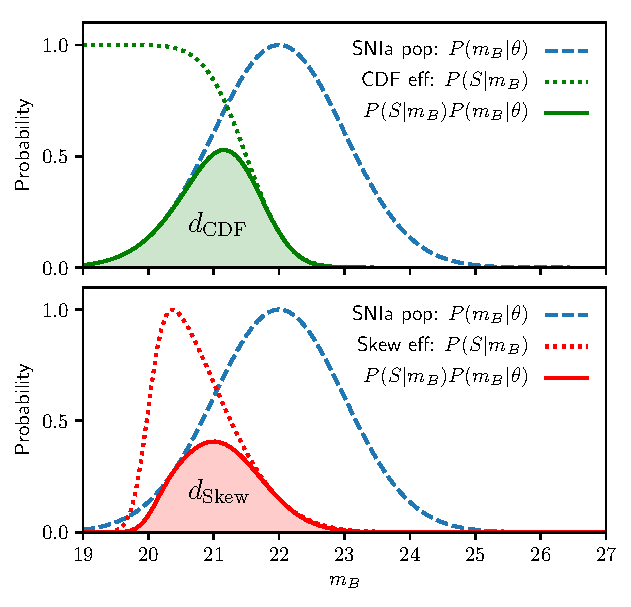
\includegraphics[width=\columnwidth]{efficiency.pdf}
	\end{center}
	\caption{The efficiency for supernova discovery at an arbitrary redshift. Shown in both panels in dashed blue is the SNIa population distribution, which takes the form of a normal distribution. The top panel shows a CDF based survey efficiency (green dotted line), whilst the bottom panel shows a skew normal based survey efficiency (red dotted line), but as generic functions of apparent magnitude. The survey efficiency, given the SNIa population, is shown as a solid line in both panels, and the probability of observing a SNIa is found by integrating over the population detection efficiency as described in equation \eqref{eq:w1}, and has been shown by shading the area integrated. This area is what is analytically given by equations \eqref{eq:seldes} and \eqref{eq:sellowz}.}
	\label{fig:efficiency}
\end{figure}






\section{Model Verification}
\label{sec:verification}

In order to verify our model we run it through several tests. First, we validate on toy models, verifying that there is not significant cosmological bias in highly constraining datasets. We then validate our model on SNANA simulations based on a collection of low redshift surveys and the DES three year spectroscopic sample.

\subsection{Applied to Toy Spectroscopic Data}
\label{sec:toy}


\begin{figure}
	\begin{center}
		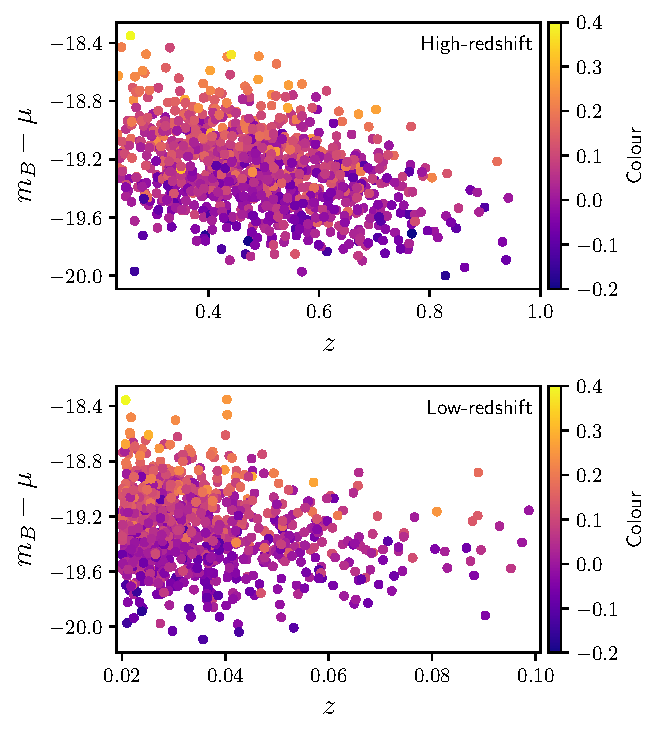
\includegraphics[width=\columnwidth]{plot_pop_simple.pdf}
	\end{center}
	\caption{Population distributions shown in redshift and uncorrected absolute magnitude $m_B - \mu$ for 1000 supernovae in both high-redshift and low-redshift surveys. Selection effects are visible in both samples, where red supernovae are often cut as redshift increases. The colour of the data points is representative over the supernovae colour itself, blue dots represent blue supernovae, with warmer colours representing redder supernovae.}
	\label{fig:simple_pop}
\end{figure}
\begin{figure}
	\begin{center}
		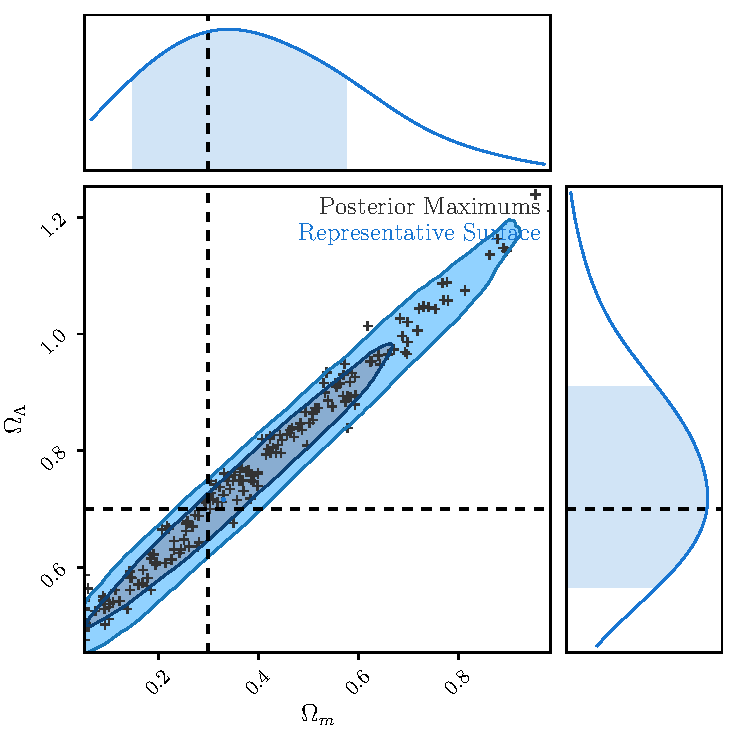
\includegraphics[width=\columnwidth]{simpleApproximateModelOl.pdf}
	\end{center}
	\caption{Maximal posterior points for 100 realisations of supernova data with the Flat $\Lambda$CDM model, with a representative contour from a single data realisation shown for context. Even a large supernova sample when treated robustly is insufficient to provide tight constraints on either $\Omega_m$ and $\Omega_\Lambda$ due to the severe degeneracy between the parameters.}
	\label{fig:simple_ol}
\end{figure}
\begin{figure}
	\begin{center}
		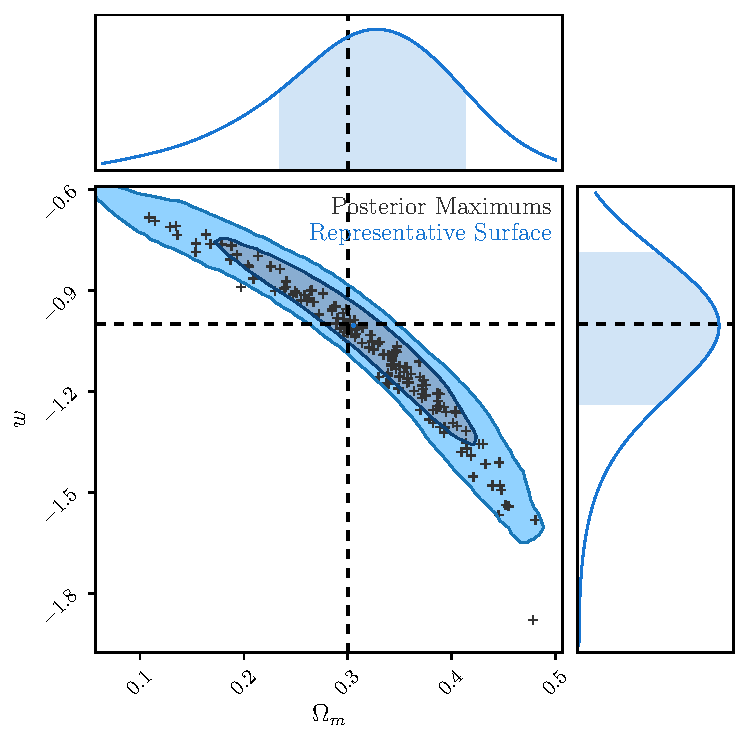
\includegraphics[width=\columnwidth]{simpleApproximateModelW.pdf}
	\end{center}
	\caption{Maximal posterior points for 100 realisations of supernova data with the Flat $w$CDM model, with a representative contour from a single data realisation shown for context. The well known banana shaped contour is recovered, with the marginalised distributions in $\Omega_m$ and $w$ providing misleading statistics due to the highly non-Gaussian nature of the posterior surface. The recovered posteior maximums show the same degeneracy direction as the representative surface and scatter around the truth values input into the simulation, shown in dashed lines.}
	\label{fig:simple_w}
\end{figure}

\begin{table}
	\centering
	\caption{Cosmological parameters determined from the surfaces of 100 fits to independent realisations of toy supernova data. As described in the main text, each dataset comprised 1000 low-redshift supernovae and 1000 high-redshift supernovae. For each chain, we record the mean and standard deviation, and then show the average mean and average standard deviations in the table. The scatter introduced by simulation variance (the standard deviation of the 100 mean parameter values) is shown in brackets. Model bias would appear as shifts away from the simulation values of $\Omega_m = 0.3$, $w = -1$. As we are using 100 independent realisations, the precision of our determination of the mean simulation result is a tenth of the quoted standard deviation: $\sqrt{100} = 10$. As the deviation from truth values is below this threshold, no significant bias is detected in either the Flat $\Lambda$CDM model or the Flat $w$CDM model (which was run with a prior on $\Omega_m$).}
	\label{tab:simple_model}
	\begin{tabular}{l|cc}
		\hline
		Model & $\Omega_m$(scatter) & $w$(scatter) \\ 
		\hline
		Flat $\Lambda$CDM & $0.301\pm 0.015(0.012)$ & -- \\ 
		Flat $w$CDM & -- & $-1.00\pm 0.042(0.030)$ \\ 
		\hline
	\end{tabular}
\end{table}

We generate simple toy data to validate the basic premise of the model. Data generation algorithm is described below:

\begin{enumerate}[1.]
	\item Draw a redshift from a power law distribution. For the low redshift survey this is $\mathcal{U}(0.0004, 0.01)^{0.5}$, and for the DES-like survey this is $\mathcal{U}(0.008, 1.0)^{0.3}$.
	\item Draw a true absolute magnitude, stretch and colour from the respective distributions $\mathcal{N}(-19.3, 0.1)$, $\mathcal{N}(0, 1)$, $\mathcal{N}(0, 0.1)$.
	\item Draw a random mass probability from $\mathcal{U}(0, 1)$ and calculate the mass-brightness correction using $\delta(0) = 0.08$ and $\delta(0)/\delta(\infty) = 0.5$ and equation \eqref{eq:mass}.
	\item Calculate $\mu(z)$ given the drawn redshift and cosmological parameters $\Omega_m = 0.3$, $w = -1$. Use this to determine the true apparent magnitude of the object $m_B$ using equation \eqref{eq:l2}.
	\item Determine if the SNIa is detected using detection probability $P(S|m_B) = \mathcal{N}^{\rm skew}(13.72, 1.35, 5.87)$ for the low redshift survey (numeric values obtained by fitting to existing low redshift data). For the DES-like survey, accept with probability $P(S|m_B) = \Phi^C(23.14, 0.5)$. Repeat from step one until we have a supernova which passes.
	\item Add independent, Gaussian observational error onto the true $m_B$, $x_1$, $c$ using Gaussian widths of $0.04$, $0.2$, $0.03$ respectively (following the mean uncertainty for DES-like SNANA simulations). Add extra colour uncertainty in quadrature of $\kappa_0 + \kappa_1 z$, where $\kappa_0 = \kappa_1 = 0.03$.
\end{enumerate}

For supernova independent uncertainty, the selection functions (a skew normal for low-redshift and an error function for high-redshift) are given independent uncertainty of $0.01$ on all parameters. We draw from each survey simulation until we have 1000 LowZ supernovae and 1000 DES-like supernovae, representing a statistical sample of greater power than the estimated 350 supernovae for the DES spectroscopic analysis. Sample data for 1000 high and low redshift supernovae are shown in Figure \ref{fig:simple_pop}, confirming the presence of strong selection effects in both toy surveys, as designed. 

We test four models: Flat $\Lambda$CDM, Flat $w$CDM, $\Lambda$CDM, and Flat $w$CDM with a prior $\Omega_m \sim \mathcal{N}(0.3, 0.01)$, with the latter included to allow sensitive tests on bias for $w$. To achieve statistical precision, we fit 100 realisations of supernovae datasets. Cosmological parameters are recovered without significant bias. Combined posterior surfaces of all 100 realisations fits for $\Lambda$CDM are shown in Figure \ref{fig:simple_ol} and fits for Flat $w$CDM are shown in Figure \ref{fig:simple_w}. By utilising the Stan framework and several efficient parametrisations (discussed further in Appendix \ref{app:optimisations}), fits to these simulations of 2000 supernovae take only on order of a single CPU-hour to run.

To investigate biases in the model in fine detail, we look for systematic bias in $\Omega_m$ in the Flat $\Lambda$CDM cosmology test, and bias in $w$ for the Flat $w$CDM test with strong prior $\Omega_m \sim \mathcal{N}(0.3, 0.01)$. This allows us to investigate biases without the investigative hindrances of non-Gaussian or truncated posterior surfaces. The strong prior on $\Omega_m$ cuts a slice through the traditional `banana' posterior surface in the $w$-$\Omega_m$ plane of Figure \ref{fig:simple_w}. Without making such a slice, the variation in $w$ can appear to be large due to a shift along the degeneracy direction of the banana. By focusing the slice at an almost fixed $\Omega_m$, we can see the variation in the mean value of $w$ approximately perpendicular to the lines of degeneracy, instead of along them. The results of the analysis are detailed in Table \ref{tab:simple_model}, and do not reveal evidence of systematic bias in our model.




















\subsection{DES SN data validation}
\label{sec:simdes}

Early analyses often treated intrinsic dispersion simply as scatter in the underlying absolute magnitude of the underlying population, but recent analyses require a more sophisticated approach. In our development of this model and tests of intrinsic dispersion, we analyse the effects of two different scatter models. The first is the \citet[][hereafter denoted {\gten}]{Guy2010} scatter model, which models intrinsic scatter with a 70\% contribution from coherent variation and 30\% from chromatic variation. The second, denoted the {\celeven} model, is sourced from \citet{Chotard2011} and has variation with 25\% contribution from coherent scatter and 75\% from chromatic variation. 

Simulations (using the SNANA package) follow the observational schedule and observing conditions for the DES and LowZ surveys, where the LowZ sample is comprised of CfA3 \citep{Hicken2009, Hicken2009a}, CfA4 \citep{Hicken2012} and CSP \citep{Contreras2010,Folatelli2010,Stritzinger2011}.


 In addition to the improvements in the scatter models over the simple data, we also include peculiar velocities for the LowZ sample, and our full treatment of systematics. Our simulated populations are sourced from \citet[][hereafter {\sk}]{Scolnic2016}. The selection effects were quantified by comparing all the generated supernovae to those that pass our simulated cuts, as shown in Figure~\ref{fig:sf_snana}. It is from this simulation that our analytic determination of the selection functions for the LowZ and DES survey are based. We note that there was no significant difference in the selection effect of Malmquist bias between using the {\gten} or {\celeven} scatter model compared to the fit uncertainty.


\begin{table}
	\centering
	\caption{Tested population distributions, where the {\sk} LowZ stretch distribution is formed as sum of two bifurcated Gaussians, with the mean and spread of each component given respectively.}
	\label{tab:dist}
	\begin{tabular}{l|cccc}
		\hline
		Model & $\langle x_1 \rangle$ & $\sigma_{x_1}$ &  $\langle c \rangle$ & $\sigma_c$  \\
		\hline
		{\sk} LowZ    &  $0.55$ \& $-1.5$ & $^{+0.45}_{-1.0}$ \& $^{+0.5}_{-0.5}$ & $-0.055$ & $^{+0.15}_{-0.023}$ \\
		{\sk} DES     & $0.973$ & $^{+0.222}_{1.472}$ & $-0.054$  &  $^{+0.101}_{0.043}$ \\
		\hline
	\end{tabular}
\end{table}




\begin{figure}
	\begin{center}
		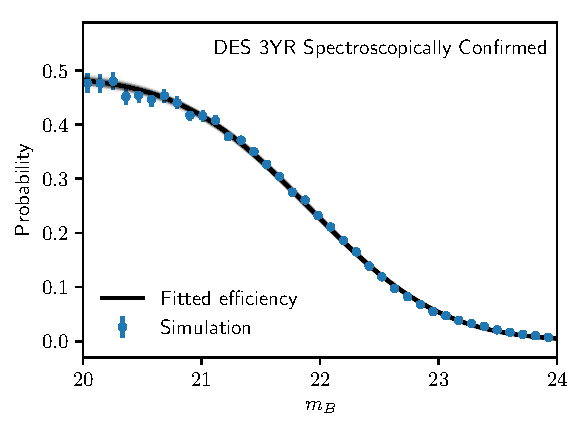
\includegraphics[width=\columnwidth]{DES3YR_DES_BHMEFF_AMG10.pdf}
		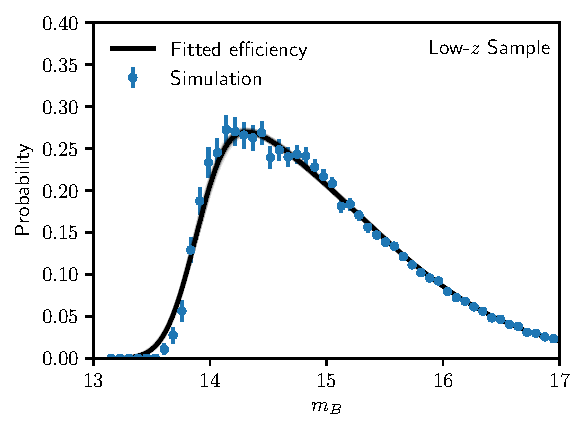
\includegraphics[width=\columnwidth]{DES3YR_LOWZ_BHMEFF_G10.pdf}
	\end{center}
	\caption{Fitting the selection function for both the DES 3YR spectroscopically confirmed supernova sample and the combined low-redshift sample. Blue errorbars represent the efficiency calculated by determining the ratio of discovered to generated supernovae in apparent magnitude bins for SNANA simulations. The black line represents the best fit analytic function for each sample, and the light grey lines surrounding the best fit value represent random realisations of analytic function taking into account uncertainty on the best fit value.}
	\label{fig:sf_snana}
\end{figure}






\begin{figure}
	\begin{center}
		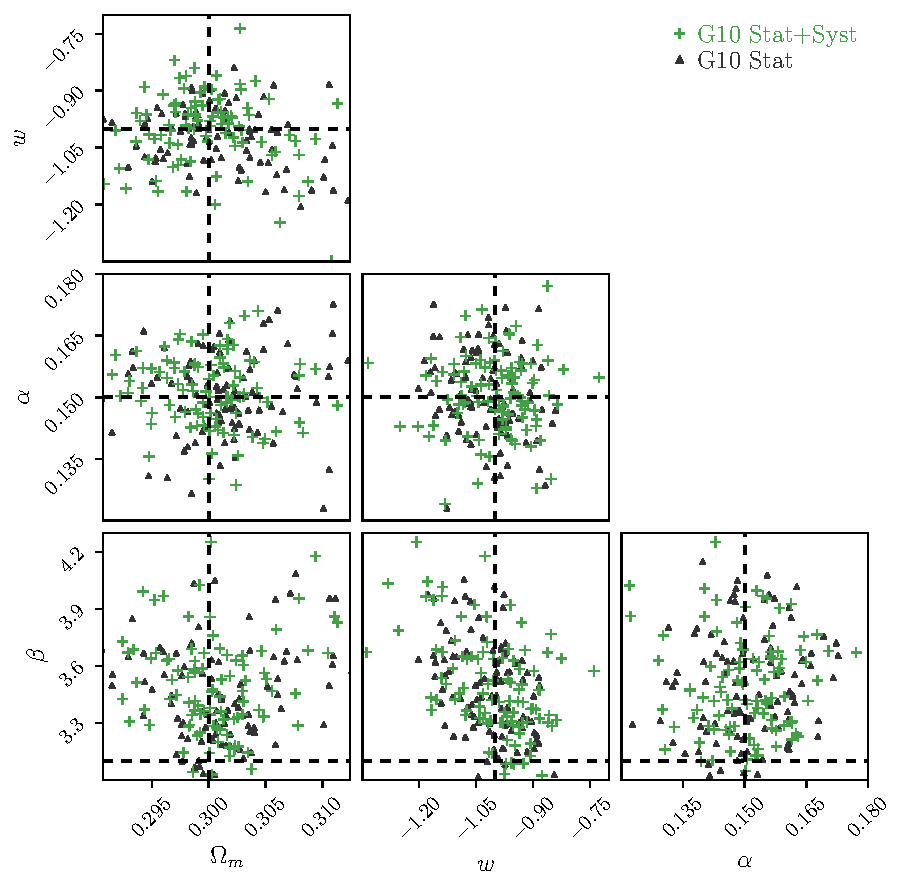
\includegraphics[width=\columnwidth]{bulk_points_g10.pdf}		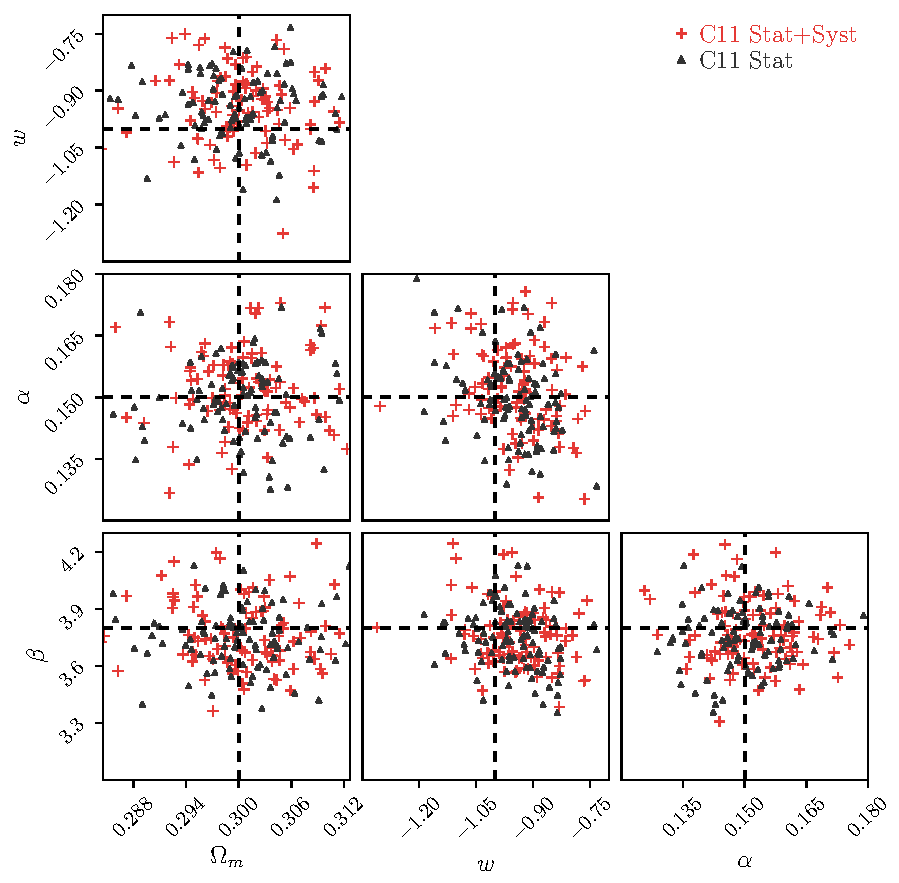
\includegraphics[width=\columnwidth]{bulk_points_c11.pdf}
	\end{center}
	\caption{Maximum posterior points for 100 realisations of supernova data for two intrinsic dispersion models - the {\gten} model for the top panel and the {\celeven} model for the bottom panel. Points are shown for parameters $\Omega_m$, $w$, $\alpha$, $\beta$ and $\langle M_B \rangle$, with the other fit parameters being marginalised over. The intrinsic scatter model has significant impact on the recovered $\beta$, which in itself effects cosmology, resulting in small biases in $w$.}
	\label{fig:bulk_posterior}
\end{figure}

\begin{table}
	\centering
	\caption{Investigating the combined 100 fits to {\gten} and {\celeven} simulations, fitting with both statistics only and also when including systematics. With systematics enabled, both the {\gten} and {\celeven} models show evidence of bias, scattering to either side of the simulated value of $w=-1$. However, their deviation from the truth value represents a shift of approximately $0.3\sigma$ when taking into account the uncertainty on fits to $w$. The bias is sub-dominant to both the size of the uncertainty for each fit, and the scatter induced by statistical variance in the simulations. }
	\label{tab:bulk_summary}
	\begin{tabular}{l|c}
		\hline
		Model & $w$ (scatter) \\
		\hline
		{\gten} Stat + Syst  &  $-1.03\pm 0.10\ (0.08)$   \\
		{\celeven} Stat + Syst  &  $-0.97\pm 0.09\ (0.06)$  \\
		{\gten}  Stat         &  $-1.01\pm 0.08\ (0.08)$   \\
		{\celeven} Stat         &  $-0.96\pm 0.07\ (0.05)$   \\
		\hline
	\end{tabular}
\end{table}


\begin{table}
	\centering
	\caption{Parameter Correlations with $w$ for the combined 100 simulation fits. Correlations for the LowZ band systematics and the latent parameters representing selection function uncertainty are not shown but have negligible correlation.}
	\label{tab:parameter_correlations}
	\begin{tabular}{c|cc}
		Parameter & {\gten} Stat+Syst & {\celeven} Stat+Syst  \\
		\hline
		$\Omega_m$ &   -0.19 &     -0.21     \\
		$\alpha$ &   -0.17 &     -0.20     \\
		$\beta$ &   -0.29 &     -0.23     \\
		$\langle M_B \rangle$ &    0.68 &      0.66     \\
		$\sigma_{\rm m_B}^{0}$ &    0.04 &      0.07     \\
		$\sigma_{\rm m_B}^{1}$ &    0.23 &      0.18     \\
		$\sigma_{x_1}^{0}$ &    0.04 &      0.03     \\
		$\sigma_{x_1}^{1}$ &    0.05 &      0.01     \\
		$\sigma_{c}^{0}$ &    0.01 &      0.11     \\
		$\sigma_{c}^{1}$ &    0.08 &      0.04     \\
		$\alpha_c^{0}$ &   -0.04 &      0.04     \\
		$\alpha_c^{1}$ &    0.03 &      0.01     \\
		$\kappa_{c0}^{0}$ &   -0.10 &     -0.05     \\
		$\kappa_{c0}^{1}$ &   -0.20 &     -0.17     \\
		$\kappa_{c1}^{0}$ &   -0.05 &     -0.01     \\
		$\kappa_{c1}^{1}$ &   -0.01 &      0.01     \\
		$s_c^{0}$ &    0.00 &      0.01     \\
		$\delta(0)$ &    0.00 &      0.00     \\
		$\delta(\infty)/\delta(0)$ &    0.00 &      0.00     \\
		$\langle x_1^{0} \rangle$ &   -0.01 &     -0.05     \\
		$\langle x_1^{1} \rangle$ &   -0.02 &      0.02     \\
		$\langle x_1^{2} \rangle$ &   -0.04 &     -0.04     \\
		$\langle x_1^{3} \rangle$ &   -0.03 &     -0.06     \\
		$\langle x_1^{4} \rangle$ &   -0.06 &     -0.06     \\
		$\langle x_1^{5} \rangle$ &    0.04 &      0.02     \\
		$\langle x_1^{6} \rangle$ &    0.04 &      0.04     \\
		$\langle x_1^{7} \rangle$ &    0.08 &      0.03     \\
		$\langle c^{0} \rangle$ &   -0.05 &     -0.12     \\
		$\langle c^{1} \rangle$ &    0.11 &      0.03     \\
		$\langle c^{2} \rangle$ &    0.11 &      0.06     \\
		$\langle c^{3} \rangle$ &    0.14 &      0.04     \\
		$\langle c^{4} \rangle$ &   -0.11 &     -0.11     \\
		$\langle c^{5} \rangle$ &   -0.15 &     -0.08     \\
		$\langle c^{6} \rangle$ &   -0.12 &     -0.13     \\
		$\langle c^{7} \rangle$ &   -0.12 &     -0.06     \\
		$\delta [ {\rm SALT}_0 ]$ &    0.05 &      0.05     \\
		$\delta [ {\rm SALT}_1 ]$ &   -0.01 &      0.02     \\
		$\delta [ {\rm SALT}_2 ]$ &   -0.10 &     -0.09     \\
		$\delta [ {\rm SALT}_3 ]$ &   -0.03 &     -0.03     \\
		$\delta [ {\rm SALT}_4 ]$ &    0.08 &      0.09     \\
		$\delta [ {\rm SALT}_5 ]$ &    0.01 &      0.02     \\
		$\delta [ {\rm SALT}_6 ]$ &    0.05 &      0.07     \\
		$\delta [ {\rm SALT}_7 ]$ &   -0.11 &     -0.10     \\
		$\delta [ {\rm SALT}_8 ]$ &    0.01 &      0.02     \\
		$\delta [ {\rm SALT}_9 ]$ &    0.02 &      0.02     \\
		$\delta [ {\rm MWE}_{B-V} ]$ &    0.03 &      0.02     \\
		$\delta [ {\rm HST Calib} ]$ &   -0.07 &     -0.07     \\
		$\delta [ v_{\rm pec} ]$ &    0.00 &     -0.01     \\
		$\delta [ {\rm \delta z } ]$ &    0.01 &      0.00     \\
		$\delta [ \Delta g ]$ &    0.05 &      0.11     \\
		$\delta [ \Delta r ]$ &    0.16 &      0.10     \\
		$\delta [ \Delta i ]$ &   -0.16 &     -0.18     \\
		$\delta [ \Delta z ]$ &   -0.26 &     -0.26     \\
		$\delta [ \Delta \lambda_g ]$ &    0.16 &      0.20     \\
		$\delta [ \Delta \lambda_r ]$ &    0.05 &      0.06     \\
		$\delta [ \Delta \lambda_i ]$ &    0.00 &     -0.01     \\
		$\delta [ \Delta \lambda_z ]$ &    0.09 &      0.07     \\
		\hline
	\end{tabular}
\end{table}


Each realisation of simulated cosmology contains 137 LowZ supernovae, and 204 DES-like supernovae, such that the uncertainties found when combining chains is representative of the uncertainty in the final DES spectroscopic analysis. As our primary focus is Dark Energy, we now focus specifically on the Flat $w$CDM model with matter prior.


 Combined posterior surfaces for 100 data realisations are shown in Figure \ref{fig:bulk_posterior}. Note that we have combined the posteriors for 100 realisations, and so we should expect the size of the uncertainty to be representative of one realisation, but the statistical spread of the final surface should be $\sqrt{100} = 10$ times less than a single realisation. The parameter bounds are listed in Table \ref{tab:bulk_summary}.
 
 
Cosmological bias is detected with $\approx 2.7\sigma$ significance for the {\celeven} model and $\approx 1.5\sigma$ significance for the {\gten} model when fitting both systematics and statistics. For the statistics only fits, the respective bias detection levels are $0.9\sigma$ and $5.5\sigma$. We investigate the {\celeven} bias and find its source to be a bias in the observed summary statistics, in addition to incorrect reported uncertainty on the summary statistics. This is confirmed by replacing the fully simulated observed $m_B$, $x_1$ and $c$ with random numbers drawn from a true Gaussian centered on the simulated SALT2 $m_B$, $x_1$ and $c$ values with covariance as reported by initial light curve fits. With this test, both the {\gten} and {\celeven} fits recover $w=-1.00$ exactly. From this, the main challenge of improving our methodology is to handle the fact that observational uncertainty is incorrect, non-Gaussian and biased. Our current model and techniques can quantify the effect of different scatter models, but being unable to constrain the `correct' (simulated) scatter model in our model fit means we cannot fully correct for the bias introduced an unknown scatter model.

Unfortunately, adding extra fit parameters to allow for shifting observables washes out cosmology, and applying a specific bias correction requires running a fiducial simulation (assuming cosmology, population and scatter model) and binning data, and is difficult to do whilst accounting for correlations with population and scatter model. This is compounded by the fact that bias corrections do not in general improve fits (increase the log posterior), and so are difficult to fit inherently. Colour bias corrections for the {\celeven} scatter model are included in our cosmology model, the strength of which are controlled by a fit parameter, $s_c$, however neither the {\gten} nor {\celeven} simulation fits constrained this parameter, and thus the majority of bias in the {\celeven} fits remain. Works such as \citet{Kessler2017} show that bias corrections can be applied to supernovae datasets that can robustly handle multiple intrinsic scatter models, and future work will center on uniting these methodologies - incorporating better bias corrections that separate intrinsic scatter bias and non-Gaussian summary statistic bias from Malmquist bias, without having to precompute standardisation parameters and populations.

\begin{figure*}
	\begin{center}
		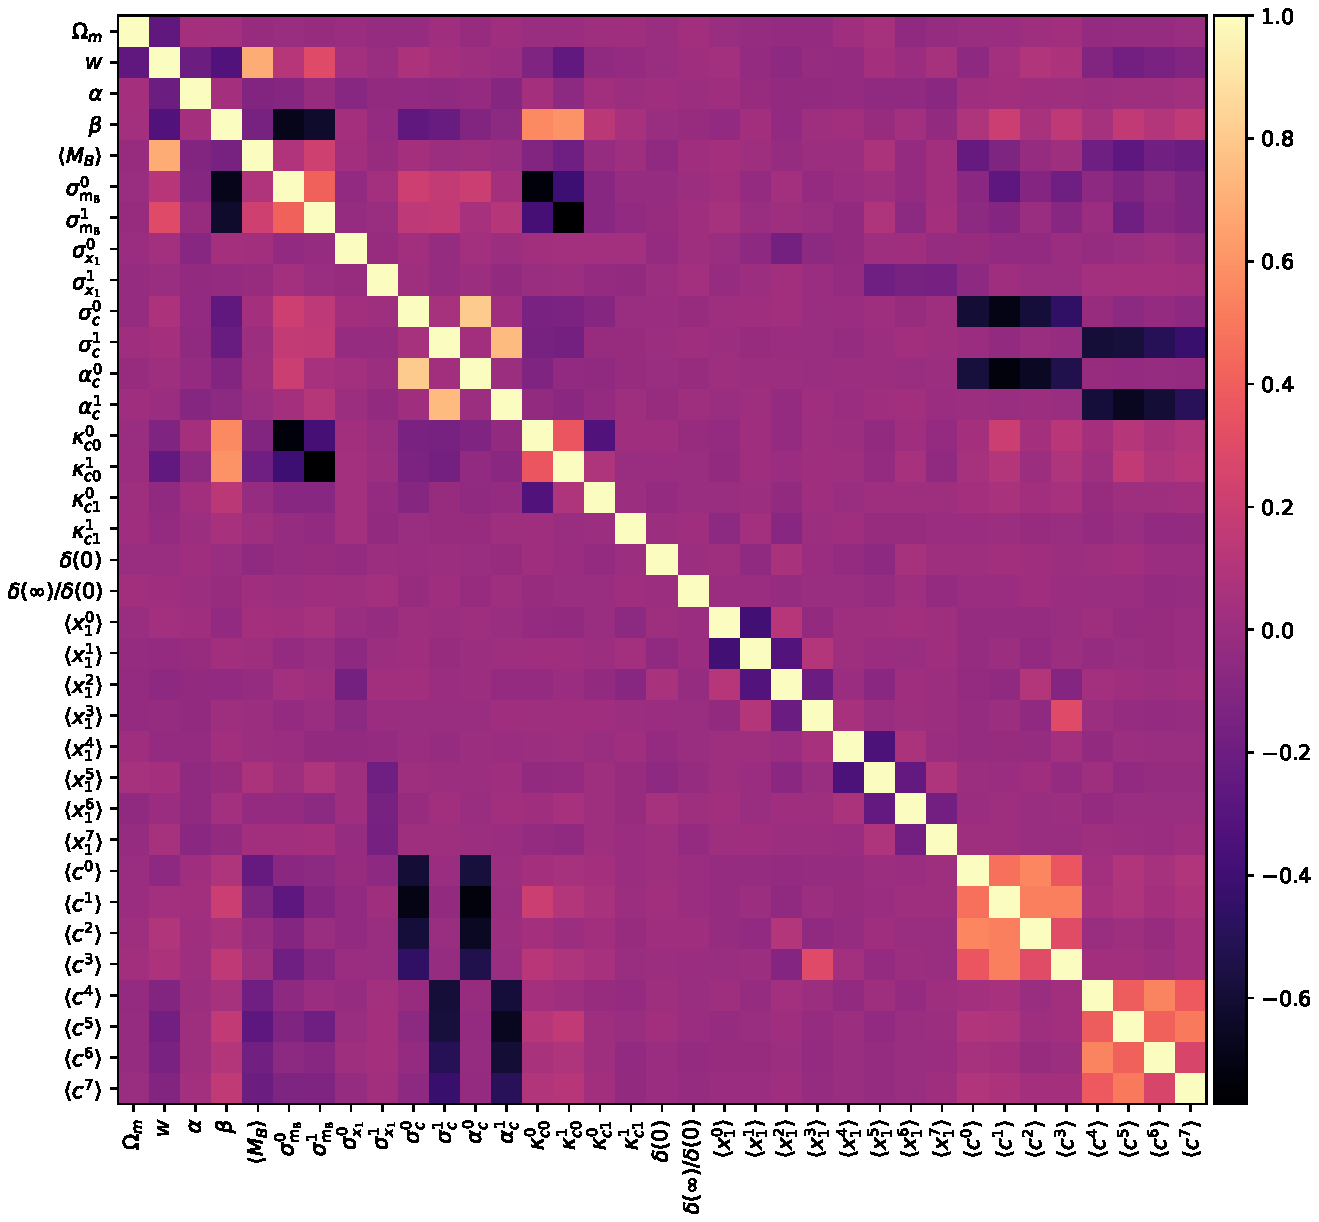
\includegraphics[width=\textwidth]{bulk_cor.pdf}
	\end{center}
	\caption{Parameter correlations for the combined fits to the 100 {\gten} scatter model simulations. We see that the primary correlations with $w$ enter through $\alpha$, $\beta$ and $\langle M_B \rangle$, as shown in Table \ref{tab:parameter_correlations}. Also visible in this figure are several other interesting relationships. $\beta$ is strongly anti-correlated with intrinsic dispersion $\sigma_{m_B}$ for both surveys (DES like and LowZ), with $\sigma_{m_B}$ showing strong anti-correlation with $\kappa^0_c$. This relationship is indeed expected - as $\kappa^0_c$ grows larger (more unexplained dispersion on the colour observation), the width of the supernova population in apparent magnitude space increases. As the fit prefers it to conform to the observed width of the distribution, the extra width in colour causes the inherent magnitude smearing amount to decrease. And with extra freedom on the observed colour from $\kappa^0_c$, $\beta$ shifts in response. The other striking feature in the plot are the strong correlation blocks in the bottom right and the anti-correlation stripes on the edges. These too are expected, for they show the relationship between the colour distributions mean value, its width and its skewness. As skewness or population width increases, the effective mean of the population shifts (see Appendix \ref{app:approx} for details), creating anti-correlation between skewness and the (Gaussian) mean colour population. Strong anti-correlation between the $\kappa_{c0}^0$ and $\kappa_{c0}^1$ (and positive fit values) shows that a finite non-zero extra colour dispersion is indeed preferred by our model.  Finally, we notice the blank cross in the middle of the figure, the result of four parameters. Firstly, the redshift-dependent extra colour dispersion for the LowZ simulation is negligible (due to the low redshift values), the bias correciton $s_c^0$ is unconstrained by our fits, and as the SNANA simulations do not include mass, we expect zero correlation across the mass step $\delta(0)$ and $\delta(\infty)/\delta(0)$ parameters. }
	\label{fig:bulk_cor}
\end{figure*}



Table \ref{tab:parameter_correlations} lists the fit correlations to our model fit parameters (excluding the LowZ band systematics, and Malmquist bias uncertainty parameters which had negligible correlation), showing (in order) cosmological parameters, standardisation parameters, population width and skewness parameters, intrinsic dispersion parameters, mass-step parameters, population mean parameters, SALT2 model systematics, dust systematic, global HST calibration systematic, peculiar velocity systematic, global redshift systematic and DES band magnitude and wavelength systematics. Figure \ref{fig:bulk_cor} show the full correlations between all non-systematic model parameters. As expected, $w$ bias is introduced primarily through incorrectly determined $\beta$, which itself is tied to the unexplained colour dispersion. Other interesting correlations are shown and discussed in Figure \ref{fig:bulk_cor}, however none have as significant an impact on cosmology as $\beta$. Table \ref{tab:parameter_correlations} does show that $\langle M_B \rangle$ is strongly correlated with $w$, however it is recovered much more accurately than $\beta$. The band systematics for DES filters $g$, $r$ and $i$ also show significant correlation with $w$, highlighting the importance of minimising instrumental uncertainty.


For the sample size of the DES and LowZ supernova samples (of order 350 supernova), the bias from intrinsic scatter models are sub-dominant to the statistical uncertainty, as shown in Figure \ref{fig:bulk_posterior}. For our full systematics model, the bias represents a deviation from $-0.15\sigma$ to $0.27\sigma$ depending on scatter model, and as such we will leave more complicated treatment of them for future work.




%		$\delta [ \Delta t ]$ &   -0.01 &      0.00     \\
%		$\delta [ \Delta y ]$ &   -0.03 &     -0.04     \\
%		$\delta [ \Delta Z ]$ &    0.10 &      0.10     \\
%		$\delta [ \Delta A ]$ &    0.00 &      0.00     \\
%		$\delta [ \Delta u ]$ &   -0.04 &     -0.03     \\
%		$\delta [ \Delta v ]$ &    0.01 &      0.02     \\
%		$\delta [ \Delta \lambda_{t} ]$ &    0.00 &      0.02     \\
%		$\delta [ \Delta \lambda_{y} ]$ &    0.00 &      0.00     \\
%		$\delta [ \Delta \lambda_{z} ]$ &   -0.05 &     -0.04     \\
%		$\delta [ \Delta \lambda_{A} ]$ &    0.00 &     -0.01     \\
%		$\delta [ \Delta \lambda_{u} ]$ &   -0.02 &     -0.02     \\
%		$\delta [ \Delta \lambda_{v} ]$ &   -0.01 &      0.01     \\
%		$\delta [ \Delta gl ]$ &   -0.12 &     -0.13     \\
%		$\delta [ \Delta hm ]$ &    0.02 &      0.01     \\
%		$\delta [ \Delta in ]$ &    0.08 &      0.13     \\
%		$\delta [ \Delta jo ]$ &    0.00 &     -0.01     \\
%		$\delta [ \Delta \lambda_{gl} ]$ &    0.00 &      0.00     \\
%		$\delta [ \Delta \lambda_{hm} ]$ &   -0.01 &     -0.03     \\
%		$\delta [ \Delta \lambda_{in} ]$ &   -0.10 &     -0.12     \\
%		$\delta [ \Delta \lambda_{jo} ]$ &    0.00 &      0.00     \\
%		$\delta [ \Delta p ]$ &   -0.01 &     -0.01     \\
%		$\delta [ \Delta q ]$ &    0.00 &      0.00     \\
%		$\delta [ \Delta R ]$ &    0.00 &      0.01     \\
%		$\delta [ \Delta s ]$ &    0.00 &     -0.01     \\
%		$\delta [ \Delta \lambda_{p} ]$ &    0.00 &      0.01     \\
%		$\delta [ \Delta \lambda_{q} ]$ &    0.01 &     -0.01     \\
%		$\delta [ \Delta \lambda_{r} ]$ &   -0.01 &     -0.01     \\
%		$\delta [ \Delta \lambda_{s} ]$ &    0.00 &      0.00     \\
%		$\delta [ \Delta b ]$ &    0.00 &     -0.01     \\
%		$\delta [ \Delta c ]$ &    0.00 &      0.00     \\
%		$\delta [ \Delta d ]$ &    0.00 &      0.01     \\
%		$\delta [ \Delta e ]$ &    0.00 &      0.00     \\
%		$\delta [ \Delta \lambda_{b} ]$ &    0.00 &     -0.01     \\
%		$\delta [ \Delta \lambda_{c} ]$ &    0.00 &      0.00     \\
%		$\delta [ \Delta \lambda_{d} ]$ &    0.00 &     -0.01     \\
%		$\delta [ \Delta \lambda_{e} ]$ &    0.00 &     -0.01     \\
%		$\Delta_{0}$ &    0.00 &      0.01     \\
%		$\Delta_{1}$ &    0.00 &     -0.01     \\
%		$\Delta_{2}$ &    0.00 &      0.00     \\
%		$\Delta_{3}$ &   -0.01 &     -0.01     \\
%		$\Delta_{4}$ &    0.00 &     -0.01     \\
%		$\Delta_{5}$ &    0.00 &     -0.01     \\
%		$\Delta_{6}$ &    0.00 &      0.00     \\
%		$\Delta_{7}$ &    0.00 &     -0.01     \\












\section{Conclusions}

In this paper we have outlined the creation of a hierarchical Bayesian model for supernova cosmology. The model takes into account selection effects and their uncertainty, fits underlying populations and standardisation parameters, incorporates unexplained dispersion from intrinsic scatter colour smearing and incorporates uncertainty from peculiar velocities, survey calibration, HST calibration, dust, a potential global redshift offset, and SALT2 model uncertainty. Furthermore, our uncertainties in standardisation, population, mass-step and more, being explicitly parametrised in our model, are captured will covariance intact, an improvement on many previous methods. The model has been optimised to allow for hundreds of supernovae to be modelled fully with latent parameters and run in under an hour of CPU time and scales linearly with the number of supernovae, as opposed to polynomial complexity of matrix inversion of other methods.

The importance of validating models using high-precision statistics gained by performing fits to hundreds of data realisations cannot be overstated, however this validation is lacking in many earlier BHM models for supernova cosmology. We have validated this model against many realisations of simplistic simulations with well-known and well-defined statistics, and found no cosmological bias. When validating using SNANA simulations, we find evidence of cosmological bias which is traced back to light curve fits reporting biased observables and incorrect covariance. Allowing fully parametrised corrections on observed supernovae summary statistics is found to make cosmology fits too weak, and allowing simulation based corrections to vary in strength is found to give minor reductions in $w$ bias, however the uncertainty on the intrinsic scatter model itself limits the efficacy of the bias corrections. For the data size represented in the DES three-year spectroscopic survey, the determined biases should be sub-dominant to other sources of uncertainty, however this cannot be expected for future analyses with larger datasets. Stricter bias corrections calculated from simulations are required to reduce bias. Ideally, this would include further work on the physical intrinsic dispersion of the Type Ia supernovae population such that we can better characterise this bias.

With our model being validated against hundreds of simulation realisations, representing a combined dataset over more than $250\,000$ simulated supernovae, we have been able to accurately determine biases in our model and trace their origin. With the current biases being sub-dominant to the total uncertainty, we now prepare to analyse the DES three-year dataset.

\section*{Acknowledgements}

Plots of posterior surfaces and parameter summaries were created with \verb|ChainConsumer| \citep{Hinton2016}.



%%%%%%%%%%%%%%%%%%%% REFERENCES %%%%%%%%%%%%%%%%%%

% The best way to enter references is to use BibTeX:

\bibliographystyle{mnras}
\bibliography{bib}




%%%%%%%%%%%%%%%%% APPENDICES %%%%%%%%%%%%%%%%%%%%%

\appendix

\section{Selection Effect Derivation}
\label{app:selection}

\subsection{General Selection Effects}

When formulating and fitting a model using a constraining dataset, we wish to resolve the posterior surface defined by
\begin{align}
P(\theta | {\rm data}) \propto P({\rm data} | \theta) P(\theta),
\end{align}
which gives the probability of the model parameter values ($\theta$) given the data.  Prior knowledge of the allowed values of the model parameters is encapsulated in the prior probability $P(\theta)$. Of primary interest to us is the likelihood of observing the data given our parametrised model, $\mathcal{L} \equiv P({\rm data} | \theta)$. When dealing with experiments which have imperfect selection efficiency, our likelihood must take that efficiency into account.  We need to describe the probability that the events we observe are both drawn from the distribution predicted by the underlying theoretical model \textit{and} that those events, given they happened, are subsequently successfully observed.  To make this extra conditional explicit, we write the likelihood of the data given an underlying model, $\theta$, \textit{and} that the data are included in our sample, denoted by $S$, as:
\begin{align}
\mathcal{L} &= P({\rm data} | \theta, S). \label{eq:app_like}
\end{align}
A variety of selection criteria are possible, and in our method we use our data in combination with the proposed model to determine the probability of particular selection criteria.  That is, we characterise a function $P(S|{\rm data},\theta)$, which colloquially can be stated as \textit{the probability of a potential observation passing selection cuts, given our observations and the underlying model}. We can introduce this expression in a few lines due to symmetry of joint probabilities and utilising that $P(x,y,z) = P(x|y,z)P(y,z) = P(y|x, z)P(x, z)$:
\begin{align}
P({\rm data} | S , \theta) P(S, \theta) &= P(S | {\rm data}, \theta) P({\rm data}, \theta)\\
P({\rm data} | S , \theta) &= \frac{ P(S | {\rm data}, \theta) P({\rm data}, \theta) }{ P(S, \theta) }\\
&= \frac{ P(S | {\rm data}, \theta) P({\rm data} | \theta) P(\theta)}{ P(S | \theta)  P(\theta)}\\
&= \frac{ P(S | {\rm data}, \theta) P({\rm data} | \theta)}{ P(S | \theta) }
\end{align}
which is equal to the likelihood $\mathcal{L}$. Introducing an integral over all possible events $D$, so we can evaluate $P(S|\theta)$, 
\begin{align}
\mathcal{L}&= \frac{P(S|{\rm data},\theta) P({\rm data}|\theta)}{\int P(S, D|\theta)\, dD} \\
\mathcal{L} &= \frac{P(S|{\rm data},\theta) P({\rm data}|\theta)}{\int P(S | D, \theta) P(D|\theta)\, dD}, \label{eq:app_main}
\end{align}
where we define the denominator as $w$ for simplicity in future derivations.



\subsection{Supernova Selection Effects}

We assume that our selection effects can be reasonably well encapsulated by independent functions of (true) apparent magnitude and redshift, such that $P(S|{\rm data}, \theta) = P(S|z) P(S|m_B)$. Our denominator then becomes
\begin{align}
d &= \int d\hat{z} \, d\hat{m}_B \, dz \, dm_B P(S|z) P(S|m_B) P(\hat{z}|z) P(\hat{m}_B|m_B) P(z, m_B | \theta), \label{eq:sel}
\end{align}
where for simplicity we have not written out all the integrals which do not interact with the selection effects explicitly. Due to our assumed perfect measurement of redshift, $P(\hat{z}|z) = \delta(\hat{z} - z)$. $P(\hat{m}_B | m_B)$ is a Gaussian due to our Gaussian model of summary statistics, and $m_B$, $x_1$, $c$, and can be analytically integrated out, collapsing the integral over $\hat{m}_B$ (which is why they were not included in equation \eqref{eq:sel}). Finally, we can express $P(z, m_B | \theta)$ as  $P(m_B | z, \theta) P(z | \theta)$, where the first term requires us to calculate the magnitude distribution of our underlying population at a given redshift, and the second term is dependent on survey geometry and supernovae rates. We can thus state
\begin{align}
d = \int \left[ \int P(S|m_B) P(m_B | z, \theta)\, dm_B \right] P(S|z)P(z|\theta)\, dz.
\end{align}
By assuming that the distribution $P(S|z)P(z|\theta)$ is well sampled by the observed supernovae redshifts, we can approximate the integral over redshift by evaluating
\begin{align}
\int P(S|m_B) P(m_B | z, \theta)\, dm_B \label{eq:selint}
\end{align}
for each supernova in the dataset -- i.e. Monte Carlo integration with assumed perfect importance sampling.

As stated in Section \ref{sec:selection}, the underlying population in apparent magnitude, when we discard skewness, can be represented as $\mathcal{N}(m_B|m_B^*(z), \sigma^*_{m_B})$, where
\begin{align}
m_B^*(z) &= \langle M_B \rangle + \mu(z) - \alpha \langle x_1(z) \rangle + \beta \left(\langle c(z) \rangle + \sqrt{\frac{2}{\pi}}\sigma_c \delta_c\right)\label{eq:disc1} \\
\sigma^*_{m_B} &= \sigma_{M_B}^2 + (\alpha \sigma_{x_1})^2 +  \left(\beta \sigma_c \sqrt{1 - \frac{2\delta_c^2}{\pi}}\right)^2. \label{eq:disc2}
\end{align}
Then, modelling $P(S|m_B)$ as either a normal or a skew normal, we can analytically perform the integral in equation \eqref{eq:selint} and reach equations \eqref{eq:seldes} and \eqref{eq:sellowz}.





\subsection{Approximate Selection Effects}
\label{app:approx}

Equations \eqref{eq:disc1} and \eqref{eq:disc2} make the assumption that, for our colour distribution, $\mathcal{N}^{\rm Skew}(\mu, \sigma, \alpha)$ is well approximated by $\mathcal{N}(\mu, \sigma)$. We sought to improve on this approximation by adjusting the mean and standard deviation of the approximated normal to match the actual mean and standard deviation of skew normal. With $\delta \equiv \alpha/\sqrt{1+\alpha^2}$, the correct mean and standard deviation are
\begin{align}
\mu_1 &= \mu_0 + \sqrt{\frac{2}{\pi}} \delta \sigma_0 \\
\sigma_1 &= \sigma_0 \sqrt{1 - \frac{2 \delta^2}{\pi}}.
\end{align}
We can then test the approximation $\mathcal{N}^{\rm Skew}(\mu_0, \sigma_0, \alpha) \rightarrow \mathcal{N}(\mu_1, \sigma_1)$. Unfortunately, this shift to the mean and standard deviation of the normal approximation did not produce stable posterior surfaces which Stan could fit when we included full covariance between $m_B$, $x_1$ and $c$ in the underlying population, and so we simplified the model to have independent parameters. Stable surfaces with underlying population covariance were found when we fixed $\sigma_c$ in the shift correction, such that $\mu_1 = \mu_0 + \sqrt{2/\pi}\delta k$, where we set $k=0.1$ to mirror the width of the input simulation population.  However, this resulted in several population parameters becoming biased, and so we do not fix $\sigma_c$. Comparing whether we shift our normal in the approximation or simply discard skewness, Figure \ref{fig:shift} shows that the calculated efficiency is significantly discrepant to the actual efficiency if the normal approximation is not shifted. The biases when using shifted or unshifted normal approximations when we fit our model on Gaussian and skewed underlying populations are shown in Figure \ref{fig:simple_w_super}, and only the shifted normal approximation correctly recovers underlying population parameters.

\begin{figure}
	\begin{center}
		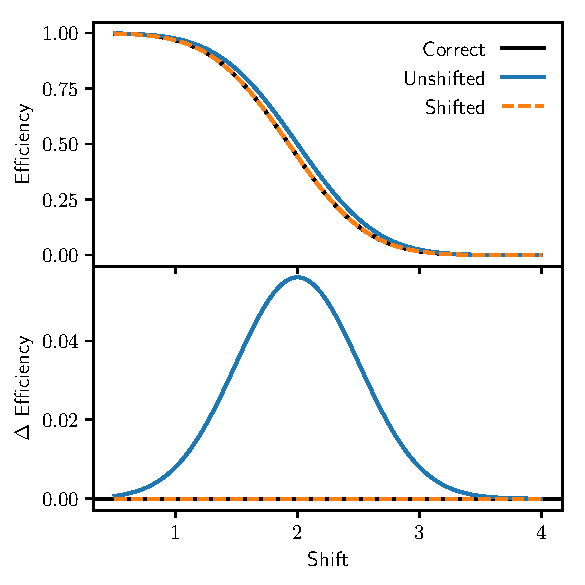
\includegraphics[width=\columnwidth]{shift.pdf}
	\end{center}
	\caption{Testing the correctness of our normal approximation to the skewed colour distribution. The `correct' line (shown in black) represents the exact integral $w = \int P(S|x) P(x) dx$ where $P(S|x)$ is an error function (following our high-redshift surveys) and $P(x) = \mathcal{N}^{\rm Skew}(x, 0.1, 2)$, calculated numerically. The $x$-axis is analogous to $m_B$ is cosmological context. As expected, all efficiencies drop towards zero as shift increases (as objects get fainter). The unshifted normal approximation shows significant discrepancy in the calculated efficiency as it transitions from 1 to 0, whilst the shifted normal approximation shows negligible error to the correct solution. From these plots, further refinement of the normal approximation (such as including kurtosis or higher powers) as unnecessary.}
	\label{fig:shift}
\end{figure}

\begin{figure*}
	\begin{center}
		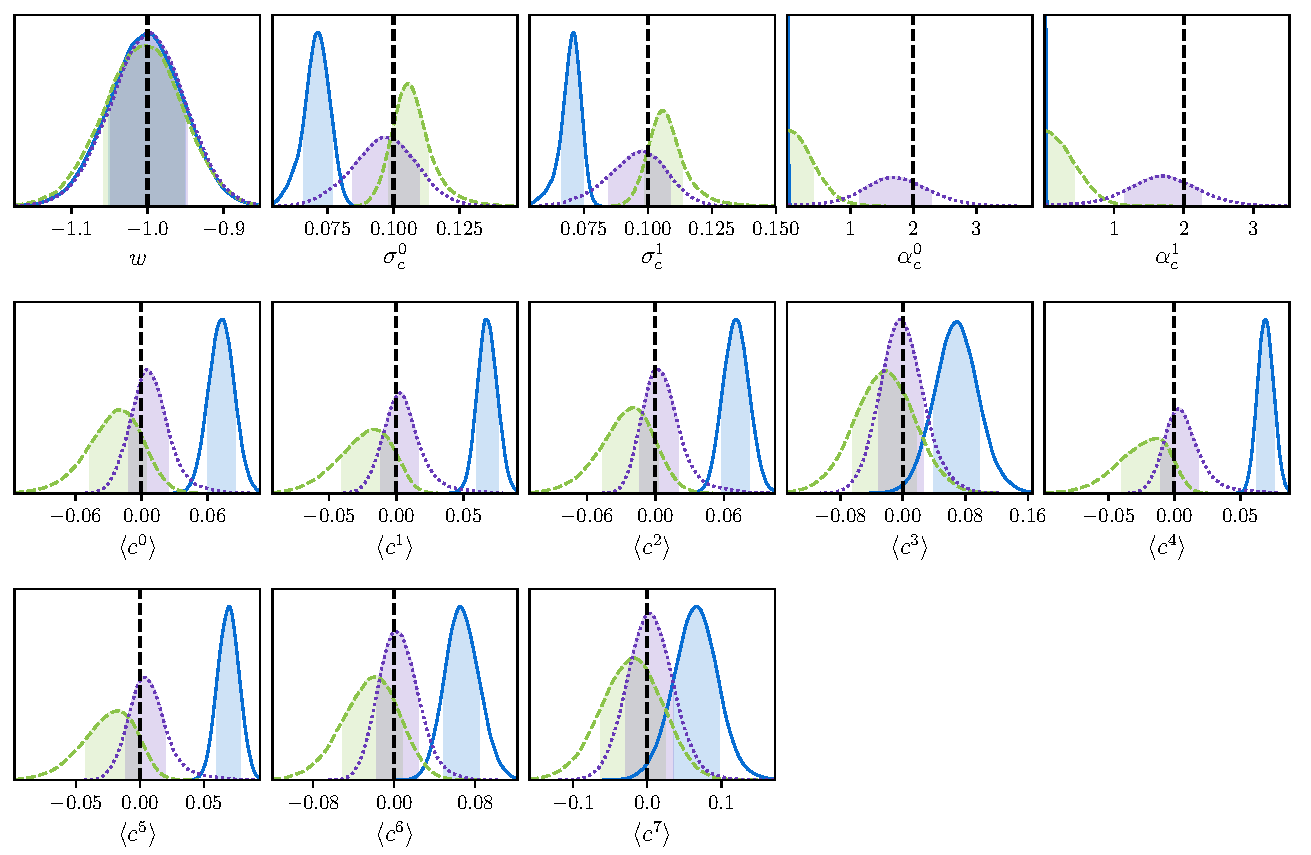
\includegraphics[width=\textwidth]{simple_w_shift_dist_0.pdf}
	\end{center}
	\caption{Marginalised probability distributions for 100 realisations of cosmology, fit to Flat $w$CDM with prior $\Omega_m \sim \mathcal{N}(0.3, 0.01)$, each containing 1000 simulated high-z and 1000 simulated low-z supernovae. The dashed green surfaces represent a fit to an underlying Gaussian colour population with the unshifted model. The blue solid surface represents fits to a skewed colour population with the unshifted model, and the purple dotted surface represents a fit to a skewed colour population with the shifted model. The superscript $0$ and $1$ denote the two different surveys (high-z and low-z respectively), and similarly the first four $\langle c^i \rangle$ parameters represent the four redshift nodes in the high-z survey, and the last four represent the nodes for the low-z survey. We can see that the shifted model is far better able to recover skewed input populations than the unshifted, performing better in terms of recovering skewness $\alpha_c$, mean colour $\langle c \rangle$ and width of the colour distribution $\sigma_c$. The unshifted model recovers the correct colour mean and width if you approximate a skew normal as a normal: $\Delta\mu = \sqrt{2/\pi}\sigma_c\delta_c \approx 0.071$, which is approximately the deviation found in fits to the colour population mean. Importantly, the unshifted model when run on skewed data (the solid blue) shows extreme bias in $\alpha_c$, where it fits strongly around zero regardless, showing it to be a poor approximation.}
	\label{fig:simple_w_super}
\end{figure*}


















\section{Numerical Optimisations}
\label{app:optimisations}


Not many fitting methodologies and algorithms can handle the thousands of fit parameters our model requires. By using Stan, we are able to take advantage automatic differentiation and the NUTS sampler, which is a class of Hamiltonian Monte Carlo samplers. Even with these advantages, early implementations of our model still had excessive fit times, with our desired sub-hour running time far exceeded. 

The simplest and most commonly found optimisation we employed was to precompute as much as possible to reduce the complexity of the mathematical graph our model is translated into to compute the surface derivatives. For example, when computing the distance modulus, redshift is encountered to various powers. Instead of computing those powers in Stan, we simply pass in several arrays of redshift values already raised to the correct power. Small changes like this however only give small results.

The primary numerical improvement we made on existing frameworks was to remove costly probability evaluations of multivariate normals. To increase efficiency, the optimum way to sample a multivariate normal is to reparameterise it such that instead of sampling $\mathcal{N}(\vec{x}|\vec{\mu}, \Sigma)$, you sample $\mathcal{N}(\vec{\delta}|0,1)$ where $\vec{x} = \vec{\mu} + L \vec{\delta}$ and $L$ is the cholesky decomposition of $\Sigma$. In this way, we can efficiently sample the unit normal probability distribution instead of sampling a multivariate normal probability distribution. Switching to this parametrisation resulted in a computational increase of an order of magnitude, taking fits for a sample of approximately 500 supernovae from roughly four hours down to thirty minutes. 

This parametrisation does come with one significant downside - inflexibility. For each step the algorithm takes, we do not recompute the cholesky decomposition of the covariance of the summary statistics - that happens once at the beginning of the model setup. If we had kept the full covariance matrix parametrisation we could modify the matrix easily - for example when incorporating intrinsic dispersion we could simple add on a secondary matrix to create an updated covariance. Using cholesky decompositions, ${\rm cholesky}(\Sigma_1 + \Sigma_2) \neq L_1 + L_2$, and so we would need to recompute the decomposition for each step, which discards most of the computational benefit just gained.

Considering a $3\times3$ matrix with cholesky decomposition
\begin{align}
L = \begin{pmatrix}
a & 0 & 0 \\ b & c & 0 \\ d & e & f \\
\end{pmatrix},
\end{align}
the original covariance matrix $\Sigma$ is given by
\begin{align}
\Sigma = \begin{pmatrix}
a^2 & ab & ad \\ ab & b^2 + c^2 & bd + ce \\ ad & bd + ce & d^2 + e^2 + f^2\\
\end{pmatrix}.
\end{align}
Now, the primary source of extra uncertainty in the intrinsic dispersion models comes from chromatic smearing, which primarily influences the recovered colour parameter, which is placed as the last element in the observables vector $\lbrace m_B, x_1, c\rbrace$. We can now see that it is possible to add extra uncertainty to the colour observation on the diagonal without having to recompute the cholesky decomposition - notice that $f$ is unique in that it is the only element of $L$ that appears in only one position in the covariance matrix. To take our covariance and add on the diagonal uncertainty for colour an extra $\sigma_e$ term, we get
\begin{align}
C = \begin{pmatrix}
\sigma_{m_B}^2 & \rho_{0,1} \sigma_{m_B} \sigma_{x_1} & \rho_{0,2} \sigma_{m_B} \sigma_c \\
\rho_{0,1} \sigma_{m_B} \sigma_{x_1} & \sigma_{x_1}^2 & \rho_{1, 2} \sigma_{x_1} \sigma_c \\
\rho_{0,2} \sigma_{m_B} \sigma_c & \rho_{1, 2} \sigma_{x_1} \sigma_c &  \sigma_c^2 + \sigma_e^2 \\
\end{pmatrix}.
\end{align}
The cholesky decomposition of this is, in terms of the original cholesky decomposition, is
\begin{align}
L = \begin{pmatrix}
a & 0 & 0 \\ b & c & 0 \\ d & e & f + g \\
\end{pmatrix},
\end{align}
where $g = \sqrt{f^2 + \sigma_e^2} - f$. This allows an easy update to the cholesky decomposition to add extra uncertainty to the independent colour uncertainty. For both the {\gten} and {\celeven} models, we ran fits without the cholesky parametrisation to allow for extra correlated dispersion (instead of just dispersion on $c$), but find no decrease in bias or improved fit statistics, allowing us to use the more efficient cholesky parametrisation.





% Don't change these lines
\bsp	% typesetting comment
\label{lastpage}
\end{document}

% End of mnras_template.tex